\documentclass[12pt,a4paper,UTF8]{ctexrep}
\usepackage{iftex}
\ifPDFTeX
  \errmessage{This project must be compiled with XeLaTeX. Please switch Overleaf compiler from pdfLaTeX to XeLaTeX.}
\fi

% Overleaf 免费版建议保持快速模式。
% 交稿前如需完整高保真编译，可把下面两项改为 false / true。
\newif\iffastdraft
\fastdrafttrue
\newif\ifusecustomfonts
\usecustomfontsfalse
\newif\ifincludeappendix
\includeappendixfalse

\iffastdraft
  \PassOptionsToPackage{draft}{graphicx}
\fi

\usepackage[left=2.54cm,right=2.54cm,top=2.54cm,bottom=2.54cm]{geometry}
\usepackage{fontspec}
\usepackage{setspace}
\usepackage{graphicx}
\usepackage{booktabs}
\usepackage{longtable}
\usepackage{array}
\usepackage{caption}
\usepackage{amsmath,amssymb}
\usepackage{listings}
\usepackage{xcolor}
\usepackage[hidelinks]{hyperref}

\ifusecustomfonts
  % 定稿模式：优先使用上传到 Overleaf 的宋体 / 黑体。
  \IfFontExistsTF{SimSun}{
    \setCJKmainfont{SimSun}
  }{
    \IfFileExists{fonts/simsun.ttc}{
      \setCJKmainfont{simsun.ttc}[Path=fonts/]
    }{
      \setCJKmainfont{FandolSong-Regular}
    }
  }
  \IfFontExistsTF{SimHei}{
    \setCJKsansfont{SimHei}
  }{
    \IfFileExists{fonts/simhei.ttf}{
      \setCJKsansfont{simhei.ttf}[Path=fonts/]
    }{
      \setCJKsansfont{FandolHei-Regular}
    }
  }
\else
  % 草稿模式：使用 TeX Live 自带中文字体，减少编译时间。
  \setCJKmainfont{FandolSong-Regular}
  \setCJKsansfont{FandolHei-Regular}
\fi
\IfFontExistsTF{Times New Roman}{
  \setmainfont{Times New Roman}
}{
  \setmainfont{TeX Gyre Termes}
}

\setstretch{1.5}
\setlength{\parindent}{2em}
\setlength{\parskip}{0pt}
\captionsetup{font={normalsize},labelfont=bf}

\lstset{
  basicstyle=\ttfamily\small,
  breaklines=true,
  columns=fullflexible,
  frame=single,
  framerule=0.3pt,
  rulecolor=\color{black!30},
  backgroundcolor=\color{black!2},
  keepspaces=true
}

\ctexset{
  chapter = {
    name = {第,章},
    number = \chinese{chapter},
    format = \centering\heiti\zihao{-4},
    aftername = \quad,
    beforeskip = 0pt,
    afterskip = 6pt
  },
  section = {
    format = \heiti\zihao{-4},
    beforeskip = 6pt,
    afterskip = 6pt
  },
  appendix = {
    name = {附录},
    number = \Alph{chapter},
    format = \centering\heiti\zihao{-4},
    aftername = \quad
  }
}

\renewcommand{\thesection}{\arabic{chapter}.\arabic{section}}
\renewcommand{\thesubsection}{\thesection.\arabic{subsection}}

\newcommand{\reportequationplaceholder}[1]{
  \begin{equation}
  \tag{#1}
  \text{[请根据 Word 原稿补录该公式]}
  \end{equation}
}

\newcommand{\reportmissingfigure}[2]{
  \begin{figure}[htbp]
  \centering
  \fbox{\parbox[c][0.22\textheight][c]{0.82\textwidth}{\centering 图 #1 暂未找到可直接复用的图片资源}}
  \caption{#2}
  \end{figure}
}

\begin{document}
\zihao{-4}
\songti

\begin{titlepage}
\centering
{\heiti\zihao{2} 2026年全国大学生信息安全竞赛\par}
\vspace{1.2cm}
{\heiti\zihao{1} 作品报告\par}
\vspace{2.4cm}
\begin{flushleft}
\zihao{-4}
作品名称：\\[0.8cm]
电子邮箱：\\[0.8cm]
提交日期：\\[0.8cm]
\end{flushleft}
\vfill
\end{titlepage}

\tableofcontents
\clearpage

\chapter*{摘要}
\addcontentsline{toc}{chapter}{摘要}
本作品面向医院侧数据与模型提供方参数同时敏感的协同推理场景，构建了一套可运行、可验证、可复现的双向隐私安全推理系统。针对传统单向隐私保护难以同时兼顾数据合规与模型知识产权保护的问题，本作品以 DynamicViT 为载体，将原始动态词元剪枝中的删除式控制流改写为固定图下可执行的密态语义，通过安全比较、安全选择与稳定排序机制，使动态剪枝能力能够进入两方安全计算链路。

在系统实现上，本作品将浏览器端本地预处理、秘密分享生成、服务端权威快检、SPU 密态前向计算与审计记录整合为端到端闭环。原始影像仅在终端侧处理，跨越信任边界后仅传输密态分片、结构化元数据与审计摘要；服务端在进入密态计算前完成协议、张量与质量摘要检查，从而避免将输入天然可信作为隐含前提。

实验结果表明，本作品在 524 张医疗验证样本上取得 92.7481\% 的阈值精度，较同仓固定结构静态对照线提升 0.7634 个百分点，较未经安全化边界重写的原始 DynamicViT 提升 17.3664 个百分点。端到端双向隐私原型在 32 条医疗部署验证样本上的平均时延为 89.06 秒/样本，双向总通信量为 84.47 GiB。系统还通过协议异常输入、重放与并发守卫等 17 类黑盒验证，为安全边界和原型可服务性提供了证据支撑。


\chapter{作品概述}
\section{背景与目标}

在医疗、金融等高敏感场景中，数据使用方通常不愿以明文形式交出原始数据，模型提供方也不愿直接暴露明文模型参数。单向隐私保护机制难以同时满足双方诉求：只强调输入侧保护会暴露模型知识产权，只强调模型侧保护则会引发数据合规风险。进一步地，若模型采用按样本动态变化的剪枝路径，则依赖明文删除、阈值比较和变长前向结构的决策链很难直接迁入安全计算图，这也是许多安全推理系统被迫退化为固定结构模型的重要原因。

本作品的设计目标不是单纯提升胸片分类精度，而是在双向隐私前提下保留动态剪枝能力，并将其落实到可运行的工程系统中。为此，本作品选择动态词元剪枝视觉 Transformer 方法 DynamicViT 作为主要载体，围绕词元打分、阈值比较、保留决策与安全执行语义之间的映射关系，完成从模型结构、协议路径到前后端控制面的联动设计。

从问题形式看，本作品研究的是一个典型的两方私有推理任务：数据持有方希望在不泄露原始影像的前提下获得分类结果，模型持有方希望在不公开模型参数与中间特征的前提下完成服务。若将原始模型记为 f、输入影像记为 x，系统需要在两方仅持有各自秘密份额的条件下近似完成 f(x) 的计算，并限制任何单方从通信内容、中间状态或动态路径中恢复对方敏感信息。该形式化目标决定了作品不能只把明文模型封装为 Web 服务，而必须重新审视动态剪枝、控制流、张量形状和审计元数据在安全计算中的暴露边界。

\section{应用场景与交付边界}

本作品面向医院侧数据与模型提供方参数同时敏感的协同推理场景，目标是在不暴露原始影像和明文模型参数的前提下完成医疗影像分类。系统的主要交付对象包括终端用户、医院侧部署环境、服务端控制面以及两方安全执行域。终端侧负责本地解码、预处理、质量评估与秘密分享生成；服务端负责协议预检、重放与并发守卫、审计落盘和密态推理调度；安全执行域负责完成双向隐私约束下的前向计算并返回最终分类结果。

本作品的交付边界不包括生产级拒绝服务防护、恶意参与方串谋对抗、输出侧隐私泄露建模以及完整的多中心部署评估。本文的重点是证明：在双向隐私约束下，动态剪枝语义能够被安全化重写，并形成可运行、可验证、可复现实验闭环。

从隐私保护推理研究脉络看，早期系统多围绕卷积网络或一般前馈模型展开，例如 SecureML[14]、GAZELLE[15]、CrypTen[16] 和 Delphi[17] 等工作已经证明，在半诚实模型下可以同时保护输入与模型参数，并将主要优化集中在线性层、激活函数和加密切换流程上。然而，当模型迁移到 Transformer 后，注意力、层归一化（Layer Normalization, LayerNorm）、高斯误差线性单元（Gaussian Error Linear Unit, GELU）和大规模矩阵乘使通信量、交互轮次与数值稳定性问题同时放大，原有方案难以直接复用到动态词元剪枝场景中。

对医疗影像任务而言，问题又比通用私有推理更复杂。一方面，医院侧原始影像具有强隐私属性，模型提供方也往往不愿公开完整参数；另一方面，胸片等视觉任务存在明显的 patch 冗余，如果为了协议简化完全退回固定结构模型，又会削弱动态剪枝在时延和通信量上的潜在优势。因此，本作品关注的不是一般意义上的“能否安全推理”，而是在双向隐私、动态边界保留与工程闭环交付三者之间建立可验证的平衡。

\section{核心贡献}

本作品的核心贡献主要体现在三个方面。第一，在算法层面，将 DynamicViT 中依赖明文控制流的删除式剪枝路径重写为固定图下可执行的密态语义，使动态词元剪枝能够进入安全计算框架。第二，在系统层面，将浏览器工作线程、服务端权威快检、重放与并发守卫以及审计链整合为完整控制面闭环，保证输入、传输和执行三个阶段的边界清晰可验证。第三，在交付层面，给出可复现的实验流程、基线对比与消融验证，使系统不仅“能跑”，而且能够说明“为什么这样设计是必要的”。

\section{相关工作与技术定位}

在隐私保护视觉 Transformer 推理方向，已有研究开始关注如何在不暴露用户输入的前提下完成密态分类任务。其中，基于秘密共享的轻量级隐私保护 ViT 推理框架 SViT 是一条具有代表性的技术路线。该工作采用两个边缘服务器协同执行安全计算协议，并围绕 ViT-B/16 的关键非线性模块构建了 SExp、SDiv、SSqrt、SLayerNorm、SSoftmax、SGeLU 等协议，在保持原始 ViT-B/16 结构不变的前提下完成安全推理[13]。对于 ViT 路线，其核心注意力计算通常可写为式（1-1）：

该类工作的主要启发在于：对于隐私保护 ViT 系统，性能优化不一定只能依赖模型压缩或结构删减，也可以通过专门设计安全算子协议来降低在线计算与通信开销。文献[13]给出的结果表明，相比 CrypTen[16]，其框架在计算效率和在线通信开销方面分别可提升约 2~6 倍和 4~14 倍，这说明“围绕算子协议进行优化”本身就是一条有效路线。

但与本作品相比，SViT 的目标和系统边界并不完全相同。SViT 更强调在固定 ViT 结构下优化安全协议效率，采用的是两个边缘服务器加可信第三方离线辅助的体系；而本作品关注的是在不引入额外可信第三方的前提下，实现面向 DynamicViT 的双向隐私推理，并将动态词元剪枝边界重写为固定图下可执行的密态语义，同时补齐浏览器工作线程、服务端权威快检与审计链闭环。因此，SViT 更适合作为本作品的相关工作与技术参照，而不是对本作品主线的直接替代。

从更长的研究脉络看，隐私保护推理最早并非围绕 Transformer 展开，而是先在卷积网络和一般前馈网络上建立问题定义与协议基础。MiniONN[25]强调将已经训练完成的神经网络转换为 oblivious neural network，使既有模型在不改训练流程的前提下进入私有推理；XONN[26]则进一步利用二值化网络与 garbled circuits 显著降低线性层代价，展示了从“直接保护现有模型”到“为安全推理重塑模型形态”的演进趋势。结合 SecureML[14]、GAZELLE[15]、Delphi[17] 与 CrypTen[16] 可以看到，早期工作已经较好解决了输入保护、线性层计算和通用推理接口等基础问题，但它们大多默认网络结构固定、中间控制流简单，尚未把样本相关动态路径视为需要重点保护的对象。

当研究对象从卷积网络转向 Transformer 后，困难的焦点也随之转移。相较卷积结构，Transformer 不仅具有更高维度的矩阵乘、更频繁的归一化与激活计算，而且其实际开销会随 token 数量显著放大。因此，Transformer 私有推理的核心不再只是“如何安全地实现已有算子”，还包括“如何让模型结构本身更适合密态执行”。这也是后续 Iron[18]、BOLT[19]、BumbleBee[7]、NEXUS[20]、THE-X[22]、MPCFormer[23] 与 SecFormer[24] 等工作持续出现的重要背景。

除 SViT[13] 外，私有推理系统还经历了从通用神经网络到 Transformer 专用协议的演进。SecureML[14]、MiniONN[25]、GAZELLE[15]、XONN[26]、CrypTen[16] 与 Delphi[17] 分别从秘密共享、混合协议、garbled circuits、系统接口与工程抽象等方面推动了通用私有推理的发展；进入 Transformer 时代后，Iron[18]首先系统性讨论了 Softmax、GELU、LayerNorm 和大矩阵乘在私有推理中的复合开销，说明 Transformer 专用协议优化是独立问题，而不是卷积网络方案的简单平移。

在固定结构安全 Transformer 推理方向，现有研究大致可以分为三类。第一类以 BOLT[19] 为代表，强调在交互式协议环境中优化矩阵乘与非线性算子，从而在保留模型精度的前提下降低通信与运行成本。第二类以 BumbleBee[7] 与 THE-X[22] 为代表，更强调对大模型或同态近似路径的系统整合，通过协议组合、算子替换和近似函数设计压缩整体执行代价。第三类则以 NEXUS[20] 和 SecFormer[24] 为代表，进一步关注交互轮次与算子形态对在线性能的影响，尝试通过非交互式执行或 SMPC 友好近似来降低实际部署成本。上述研究虽然路线不同，但共同前提是模型结构大体固定，优化重点仍然落在算子与协议层。

另一类与本作品关系更直接的研究来自明文高效视觉 Transformer 领域。DynamicViT[2] 通过逐阶段词元打分和删除式稀疏化降低后续层计算量；EViT[27] 通过保留高关注 token 并融合低关注 token 来减少冗余计算；A-ViT[28] 借助自适应停止机制使不同 token 在不同深度提前退出；ToMe[29] 则通过 token merging 在几乎不改训练流程的前提下提高吞吐；MPCViT[3] 进一步把“模型结构是否适合 MPC 执行”显式纳入搜索目标。这些方法说明，视觉 Transformer 的效率问题与 token 数量管理高度相关，但它们默认剪枝、融合、停止或合并决策可以在明文环境下直接观察和执行。

正因为如此，明文高效 ViT 方法通常不能无改动地迁移到私有推理场景。无论是删除 token、让 token 提前停止，还是合并相似 token，本质上都涉及数据相关路径选择、变长结构或显式 importance 排序；若直接在安全执行域外部完成这些操作，就可能泄露输入分布、模型偏好甚至部分中间状态；若完全保留原始明文逻辑，又会使密态图难以固定、通信量和比较开销迅速上升。CipherPrune[21] 开始把词元重要性差异直接纳入私有推理优化目标，通过密态渐进式剔除低重要性词元并配合不同强度的多项式近似，同时缓解 token 数量和非线性算子开销带来的双重成本。与这些工作相比，本作品并不试图重建一套新的通用 Transformer 近似体系，而是选择以医疗影像 DynamicViT 为具体载体，把删除式词元剪枝安全化重写为 keep-mask 驱动的固定图语义，并在两方 SPU 执行、浏览器本地分片、服务端权威快检与审计闭环之间保持一致的工程边界。

综合来看，现有相关工作大致可分为三条路线：一是以 SecureML、MiniONN、GAZELLE、XONN、Delphi 和 CrypTen 为代表的通用私有推理系统，重点解决基础协议与通用神经网络算子问题；二是以 Iron、BOLT、BumbleBee、NEXUS、THE-X、MPCFormer、SecFormer 为代表的固定结构 Transformer 私有推理路线，重点降低 attention 及非线性算子的密态执行开销；三是以 DynamicViT、EViT、A-ViT、ToMe 和 CipherPrune 为代表的 token 稀疏化或动态推理路线，重点减少后续层 token 规模。本作品位于后两条路线的交叉点：它既继承了视觉 Transformer 动态 token 管理的建模思想，又必须满足两方私有推理的固定图与边界保护约束，因此研究重点不是单纯复现某一条现成方案，而是在动态剪枝、双向隐私与工程闭环之间完成兼容性重写。


\chapter{系统设计}
\section{总体架构}

系统由医院终端、本地浏览器工作线程、跨域传输通道、业务侧前置网关、服务端权威快检层和两方安全执行域共同组成。明文图像仅在浏览器工作线程中完成解码、裁剪、归一化、数据质量评估与分片生成，跨越信任边界后仅传输密态分片（share）、结构化元数据和审计摘要；服务端在进入 SPU 计算前完成协议与张量合法性检查，随后由两方安全执行链路联合输出最终分类结果。

图 2-1 采用按信任边界分区的部署拓扑：左侧为医院终端与本地明文处理域，中间为广域网与隔离缓冲区（wide area network / demilitarized zone, WAN/DMZ）传输边界，右侧为业务侧前置网关、服务端权威快检层与参与方安全执行域。图中显式标注了明文终止点和密态分片生成起点，并以差异化图例区分本地明文处理与跨边界密态通信。

\begin{figure}[htbp]
\centering
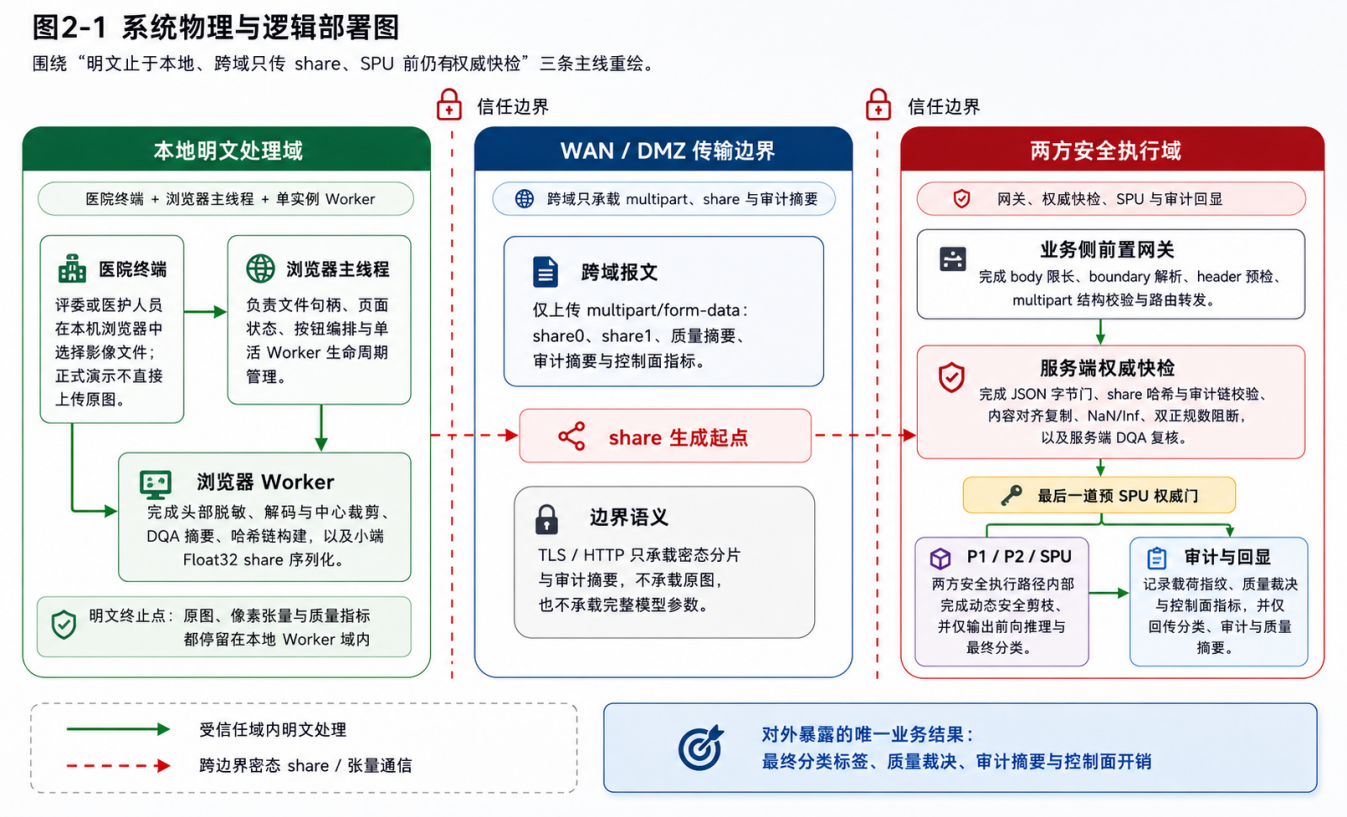
\includegraphics[width=0.92\textwidth]{figures/fig2-1-system-topology.png}
\caption{图2-1 系统物理与逻辑部署图：绿色实线表示本地明文处理，红色虚线与锁图标表示跨越信任边界的密态分片与张量通信。}
\end{figure}

\section{软件流程}

图 2-2 给出了完整的软件流转时序。主线程仅负责本地影像加载、预览和请求编排；浏览器工作线程独立完成图像解码、裁剪、数据质量评估指标提取、审计链构建与分片序列化；服务端首先执行原始报文体、边界参数、报文头与多部件结构校验，再对结构化元数据、密态分片与重构张量进行权威快检，全部通过后方可进入 SPU 密态前向计算。最终结果回传时同时包含分类结论、质量裁决、审计摘要与控制面开销，使展示链路与安全链路保持一致。

\begin{figure}[htbp]
\centering
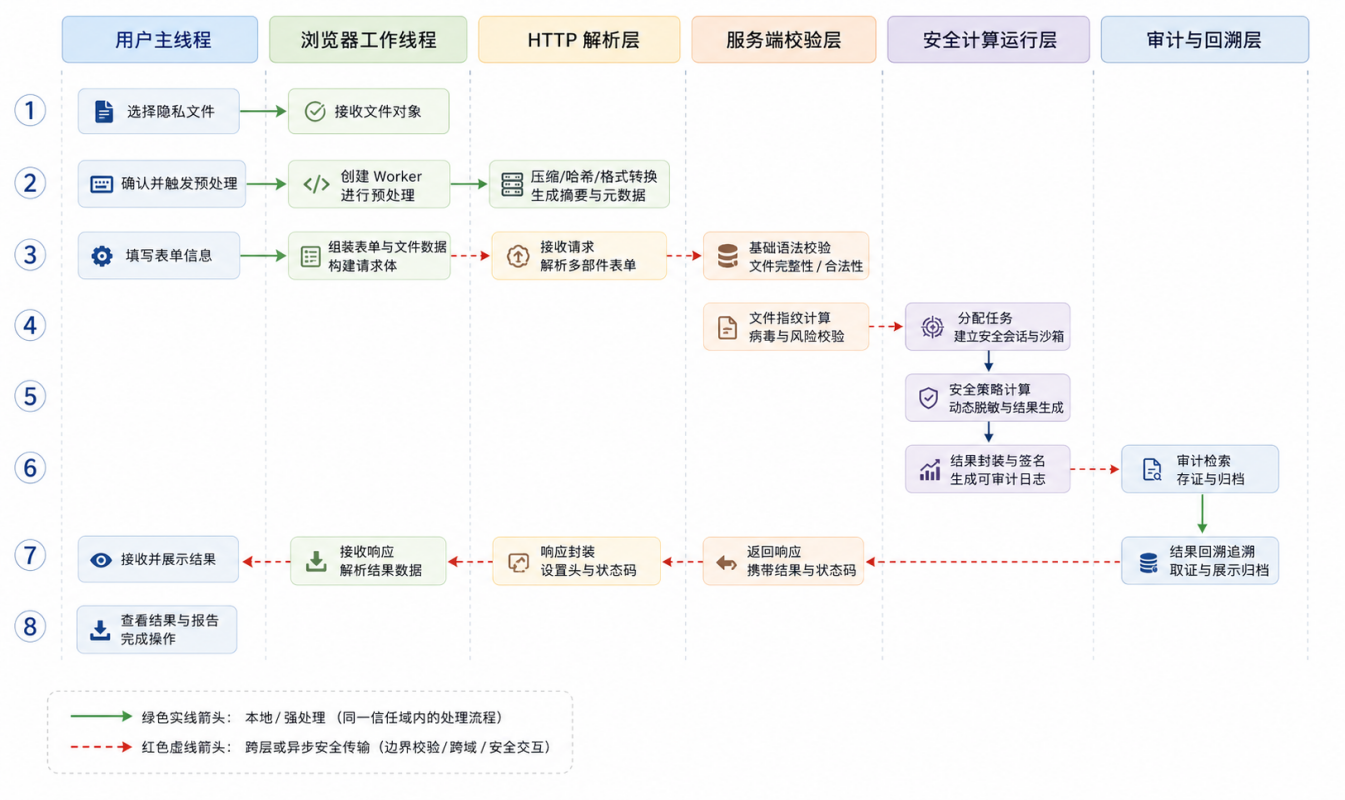
\includegraphics[width=0.92\textwidth]{figures/fig2-2-software-sequence.png}
\caption{图2-2 端到端软件流转时序图：明文仅停留在浏览器工作线程域内，跨域仅传输密态分片与审计摘要。}
\end{figure}

\section{威胁模型与安全边界}

本作品采用两方半诚实威胁模型。系统中，医院终端持有原始输入数据，模型持有方与协同计算方分别持有安全执行域中的不同份额。参与方均遵循协议执行，但可能试图从交互过程中推断对方的隐私信息。系统假设两方不串谋，且不考虑恶意篡改协议、主动注入畸形中间值或侧信道攻击等更强对抗情形。

本作品保护的对象包括：原始影像、模型参数、中间特征、动态剪枝路径以及最终推理结果；系统允许暴露的对象仅包括最小必要的结构化元数据、审计摘要和最终分类结论。本文不声称覆盖生产环境中所有攻击面，尤其不覆盖恶意共谋、模型抽取、物理侧信道和输出反推风险。系统的威胁模型、保护对象与安全边界核心定义如表 1 所示。

\begin{longtable}{>{\raggedright\arraybackslash}p{0.48\textwidth}>{\raggedright\arraybackslash}p{0.48\textwidth}}
\caption{表 1 系统威胁模型与安全边界定义}\\
\toprule
\textbf{项目} & \textbf{说明} \\
\midrule
\endfirsthead
\toprule
\textbf{项目} & \textbf{说明} \\
\midrule
\endhead
保护对象 & 用户输入数据、模型参数、中间动态决策状态、审计与控制面证据 \\
参与方 & 医院终端浏览器、浏览器工作线程、业务侧前置网关、服务端快检模块、两方 SPU 节点 \\
攻击者能力 & 可监听网络、构造畸形多部件表单报文（multipart/form-data）、伪造结构化元数据、重放一次性随机标识（nonce）、提交异常密态分片、实施并发探测 \\
安全假设 & 两方半诚实；不引入额外可信第三方；前端不作为可信根，关键裁决以服务端复算为准 \\
不覆盖范围 & 恶意参与方串谋、浏览器被完全控制、进入长耗时 SPU 后的主动断连感知、生产级分布式 DoS、防输出反演攻击 \\
防护证据 & 协议层模糊测试、重放与并发守卫测试、服务端张量快检与审计落盘证据 \\
\bottomrule
\end{longtable}

\noindent\textit{注：本表格基于两方半诚实威胁模型制定，仅覆盖原型系统设计范围内的安全假设与防护边界，不代表生产级系统的完整安全承诺}

\begin{longtable}{>{\raggedright\arraybackslash}p{0.32\textwidth}>{\raggedright\arraybackslash}p{0.32\textwidth}>{\raggedright\arraybackslash}p{0.32\textwidth}}
\caption{表 2 系统各维度安全边界覆盖情况}\\
\toprule
\textbf{边界项} & \textbf{当前覆盖} & \textbf{当前不覆盖或限制} \\
\midrule
\endfirsthead
\toprule
\textbf{边界项} & \textbf{当前覆盖} & \textbf{当前不覆盖或限制} \\
\midrule
\endhead
输入明文保护 & 明文图像只在浏览器工作线程内解码、裁剪与分片，服务端仅接收密态 share 与结构化元数据 & 不覆盖浏览器被完全控制或本地终端失陷后的明文窃取 \\
模型参数保护 & 模型参数不向数据使用方以明文暴露，仅在两方安全执行域内参与计算 & 不覆盖恶意参与方串谋、模型抽取与生产级侧信道分析 \\
动态决策隐私 & PredictorLG、阈值判断与并列分数决断保留在安全执行域内 & 不覆盖进入安全图后的主动任务取消、长连接断开感知与更强攻击模型 \\
协议与输入防护 & 原始多部件表单预检、JSON（JavaScript Object Notation）字节门、share 哈希与张量合法性快检、重放与并发守卫已落地 & 不覆盖生产级分布式 DoS、跨节点全局限流与外部 WAF/网关联动 \\
审计与复现 & nonce、请求载荷（payload）、质量摘要与审计事件落盘，报告与脚本可回溯 & 不覆盖长期合规归档平台、外部 SIEM 集成与跨系统追责链 \\
\bottomrule
\end{longtable}

\noindent\textit{注："当前覆盖" 项均已通过黑盒验证并留存审计证据；"当前不覆盖或限制" 项为原型系统明确不承诺的防护能力，需在生产部署中补充对应机制。}

各维度安全边界的具体覆盖情况与明确未覆盖范围如表 2所示，上述边界说明用于避免将原型级控制面夸大为生产级防御体系。更完整的未覆盖范围、输出侧风险与原型部署边界，统一放在第 5.5 节“当前局限性”中说明。

为便于从步骤层面概括端到端链路，算法1给出本作品从终端预处理、秘密分享、服务端预检到密态推理与结果回传的完整流程。该流程与图2-2所示时序一致，强调了明文仅停留在终端侧、跨域仅传输密态分片与审计摘要的边界约束。

从部署视角看，威胁模型不仅决定密码学协议选择，也决定系统哪些组件能够接触明文、哪些组件只能处理密态分片。许多系统只在算法层声明“保护输入与模型”，但不进一步说明原始文件、预处理张量、结构化元数据和审计记录分别落在何处。本作品在威胁模型中显式规定：原始影像与明文像素止于终端侧，跨边界传输对象被限制为 share、结构化元数据和审计摘要，服务端仅在全部快检通过后触发安全执行。这种“边界先于协议”的约束，是后续控制面设计和部署骨架成立的前提。

在安全边界之外，系统还需要处理“元数据最小化”问题。实际部署时，完全隐藏所有运行状态并不现实，因为服务端需要依据尺寸、哈希、质量摘要和任务标识完成预检、去重、审计与资源调度；但如果元数据过多，又可能间接泄露输入分布或动态路径。本作品采用最小必要原则，只保留验证任务完整性和运行可追溯所需的结构化字段，并将原始像素、明文张量、模型权重和剪枝决策限制在相应安全边界内。该设计为后续从本机展示样例迁移到医院侧与模型提供方分离部署提供了统一约束。

\section{DynamicViT 密态改写}

原始 DynamicViT 中四类核心操作的安全计算困难点、本作品的改写方案、代价与验证方式如表 3 所示。

\begin{longtable}{>{\raggedright\arraybackslash}p{0.19\textwidth}>{\raggedright\arraybackslash}p{0.19\textwidth}>{\raggedright\arraybackslash}p{0.19\textwidth}>{\raggedright\arraybackslash}p{0.19\textwidth}>{\raggedright\arraybackslash}p{0.19\textwidth}}
\caption{表 3 DynamicViT 原始操作与密态语义改写对照表}\\
\toprule
\textbf{原始DynamicViT操作} & \textbf{安全计算困难} & \textbf{本作品改写方式} & \textbf{代价} & \textbf{验证方式} \\
\midrule
\endfirsthead
\toprule
\textbf{原始DynamicViT操作} & \textbf{安全计算困难} & \textbf{本作品改写方式} & \textbf{代价} & \textbf{验证方式} \\
\midrule
\endhead
直接删除 token & 变长结构难以进入固定图安全执行，且会暴露路径 & 改写为保留/置零的掩码化表达（keep/zero），由安全选择完成保留决策 & 保留了部分冗余计算 & 本地明文参考路径与 secure replay 一致性对齐 \\
明文阈值比较 & 数据相关分支会泄露剪枝边界 & 将比较逻辑改写为安全比较语义 & 增加比较通信与控制流复杂度 & 部署阈值回代与输出一致性验证 \\
数据相关 Top-选择 & 动态索引与并列分数处理不稳定 & 采用编码索引跟踪与排序网络构造保留掩码（keep-mask） & 排序代价上升 & 排序结果与后续决策链功能验证 \\
外部明文决定 keep-mask & 会退化为半隐私运行 & 将 PredictorLG、阈值判断和并列分数决断（tie）保留在安全执行域内 & 图规模扩大、执行时间增长 & 双向隐私运行链与前端控制面联调 \\
\bottomrule
\end{longtable}

\noindent\textit{注：所有改写操作均在 SecretFlow SPU 0.9.3.dev20241118 框架下实现，验证方式包含本地明文参考对齐与密态执行一致性校验。}

为便于从工程层面理解本节中的协议友好重写，图 2-3 将原始 DynamicViT 的删除式剪枝路径与本作品的掩码化密态语义重写并列展示。其核心差异在于：正式交付链路不再直接删除词元，而是以 keep-mask 表达保留边界，从而在固定图安全执行约束下保留动态剪枝能力。

\begin{figure}[htbp]
\centering
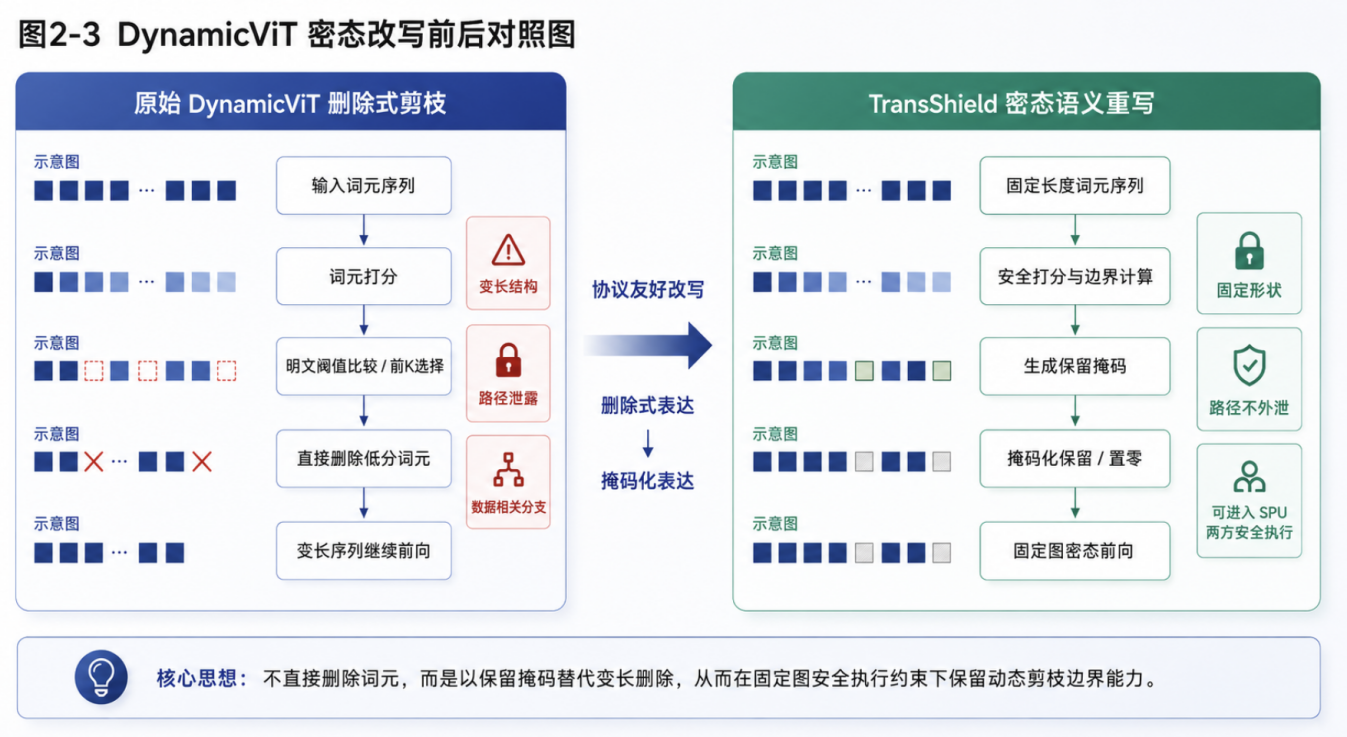
\includegraphics[width=0.92\textwidth]{figures/fig2-3-pruning-rewrite.png}
\caption{图2-3 DynamicViT 密态改写前后对照图：左侧为原始删除式剪枝，右侧为本作品的掩码化重写与固定图密态前向。}
\end{figure}

\section{硬件部署与软件基准}

本作品所有实验与性能测试均在统一的硬件与软件环境下执行，具体配置基准如表 4 所示。

\begin{longtable}{>{\raggedright\arraybackslash}p{0.48\textwidth}>{\raggedright\arraybackslash}p{0.48\textwidth}}
\caption{表 4 原型系统硬件部署与软件环境基准}\\
\toprule
\textbf{项目} & \textbf{配置} \\
\midrule
\endfirsthead
\toprule
\textbf{项目} & \textbf{配置} \\
\midrule
\endhead
CPU & Intel Xeon Gold 6148 @ 2.40GHz，80 逻辑核（2 路，每路 20 核，超线程开启） \\
物理内存 & 62 GiB \\
操作系统 & Ubuntu 20.04.6 LTS \\
内核版本 & Linux 5.15.0-139-generic \\
Python & Python 3.9.25 \\
安全计算底座 & SecretFlow SPU 0.9.3.dev20241118（Apache License 2.0） \\
原型运行模式 & 两方 2PC colocated localhost 原型链路，通信量来自同配置 fresh rerun 的 SPU LinkDetails 计数器 \\
GPU & 服务器侧配备 4 张 NVIDIA GeForce RTX 3090 GPU，单卡显存 24576 MiB（约 24 GiB），驱动版本为 570.133.07，CUDA 版本为 12.8。 \\
\bottomrule
\end{longtable}

需要说明的是，表 4 记录的是当前原型系统在统一软件栈和统一硬件条件下的实验基准，而不是医院生产环境的最终配置。安全推理时延同时受到协议轮次、矩阵规模、底层数值库、并发方式和网络条件影响；若脱离统一环境去比较动态主线、静态基线与外部相关工作，结论容易失真。因此，后续章节中出现的通信量、端到端时延和鲁棒性指标，均默认建立在本节给出的统一基准之上。

\section{展示样例与真实部署框架}

为区分原型演示与后续部署边界，本作品在工程实现中将系统形态划分为“本机展示样例”和“真实部署框架”两类。本机展示样例用于验证端到端流程：系统在一台机器上启动本地双节点安全处理器单元（Secure Processing Unit, SPU），由展示站前端完成图像选择、预处理与分片生成，后端完成协议校验、审计记录和密态前向计算，形成可运行、可追踪的闭环。

真实部署框架面向医院侧与模型提供方分离部署。该框架保留了 public manifest、P1/P2 party manifest、单方 share 加载、远程 2PC 配置生成、医院侧/AI 侧/协调侧三类网关角色以及部署包生成脚本。医院侧负责原始影像接收、预处理与 P1 share 留存，AI 或模型提供方负责 P2 share 与模型 manifest 管理，协调侧负责公开任务状态、运行编排和最终可公开结果的返回。

二者对应同一安全推理思想下的不同交付层次：本机展示样例证明流程可运行、可审计、可复现；真实部署框架提供向两方部署迁移的接口、配置和脚本骨架。当前框架提供的是部署迁移基础，不直接覆盖生产环境中的医院 HIS/PACS 接入、机构身份认证、TLS/VPN、长期审计、任务队列、密钥管理和模型私有加载策略，相关内容需要在具体医院与模型提供方环境中按现场规范继续集成。


\chapter{系统实现}
\section{模型改造与两方安全推理链路}

模型实现遵循“明文训练、密态执行语义重写、双向隐私推理落地”三层结构。训练阶段保留 DynamicViT 的词元打分与样本级动态边界能力；部署阶段将删除式剪枝语义改写为固定图可执行的掩码化表达；推理阶段由 SPU 与 OpenBumbleBee 两方安全推理集成层承担密态执行，仅对外返回最终分类结果。该实现路径的目标不是复现一条完全等价的可变长明文执行图，而是在固定图安全执行约束下尽可能保留动态剪枝边界的判别价值。

对应到动态词元剪枝的核心计算关系，医疗动态安全剪枝链路不再直接删除词元，而是先确定当前 stage 的保留边界，再生成固定形状的 keep-mask，并据此完成后续安全选择。关键关系见式（3-1）至式（3-2e）：

\begin{equation}
\tau^{(l)}=\operatorname{TopKBoundary}\!\left(s^{(l)},K^{(l)}\right), \quad m_i^{(l)}=\mathbf{1}\!\left[\left(s_i^{(l)},i\right)\ge \tau^{(l)}\right]
\tag{3-1}
\end{equation}

\begin{equation}
\tilde{h}_i^{(l)}=m_i^{(l)} \cdot h_i^{(l)}
\tag{3-2}
\end{equation}

\begin{equation}
e_i^{(l)}=s_i^{(l)}-\epsilon \cdot i
\tag{3-2a}
\end{equation}

\begin{equation}
\pi^{(l)}=\operatorname{BitonicSortDesc}\!\left(e^{(l)}\right), \quad m_i^{(l)}=\mathbf{1}\!\left[i\in \pi^{(l)}_{1:K^{(l)}}\right]
\tag{3-2b}
\end{equation}

其中，$s^{(l)}$ 表示第 $l$ 个剪枝 stage 的词元得分向量，$K^{(l)}$ 表示该 stage 允许保留的词元数，$\tau^{(l)}$ 表示由排序边界导出的保留阈值，$e_i^{(l)}$ 表示引入索引微扰后的编码键，$\pi^{(l)}$ 表示经编码键双调排序得到的索引排列，$m_i^{(l)}$ 表示第 $i$ 个词元的保留掩码。报告正文中的安全选择原语 $F_{\text{mux}}$ 与安全比较原语 $F_{\text{less}}$ 正是围绕这组关系完成的协议友好改写。

式（3-2a）与式（3-2b）对应当前密态执行中的并列分数稳定化策略：先通过编码键将词元得分与索引绑定，再在固定比较网络中执行按索引跟踪的双调排序，最后直接从排序结果的前个索引构造 keep-mask。这样做避免了“先排序求阈值、再对全体词元执行一次阈值比较”的二次密态比较开销，同时保证并列分数情况下的保留决策具有确定性。

\begin{equation}
K^{(l)}=\left\lceil \rho^{(l)} N^{(l)} \right\rceil, \quad N_{\text{out}}^{(l)}=\sum_{i=1}^{N^{(l)}} m_i^{(l)}
\tag{3-2c}
\end{equation}

\begin{equation}
b_i^{(l)}=F_{\text{less}}\!\left(\tau^{(l)}, s_i^{(l)}\right)
\tag{3-2d}
\end{equation}

\begin{equation}
\tilde{h}_i^{(l)}=F_{\text{mux}}\!\left(b_i^{(l)}, h_i^{(l)}, 0\right)
\tag{3-2e}
\end{equation}

式（3-2c）进一步给出每个剪枝 stage 的保留预算约束；式（3-2d）与式（3-2e）则分别把保留判定与安全选择写为 $F_{\text{less}}$ 和 $F_{\text{mux}}$ 原语。其中，$\rho^{(l)}$ 表示第 $l$ 个阶段的目标保留率，$N^{(l)}$ 表示该阶段输入词元数，$N_{\text{out}}^{(l)}$ 表示 keep-mask 作用后的实际保留词元数，$b_i^{(l)}$ 表示第 $i$ 个词元在该阶段的安全比较结果。

考虑到本作品的核心创新在于将 DynamicViT 的删除式剪枝重写为固定图下可执行的 keep-mask 语义，算法2进一步给出动态词元剪枝的安全化执行步骤。该算法与式（3-1）至式（3-2e）一一对应，用于说明词元打分、编码排序、保留掩码构造与安全选择之间的实现关系。

图 3-1 从实现结构角度补充展示当前项目框架：上层对应医院终端、业务网关与双节点密态执行域；中层分别对应控制面闭环、DynamicViT 安全化重写组件与两方半诚实安全计算协议；底层则是秘密分享、比较/选择与审计摘要等密码学基础原语。该图用于说明第 2 章“系统设计”与第 3 章“系统实现”的衔接关系。

\begin{figure}[htbp]
\centering
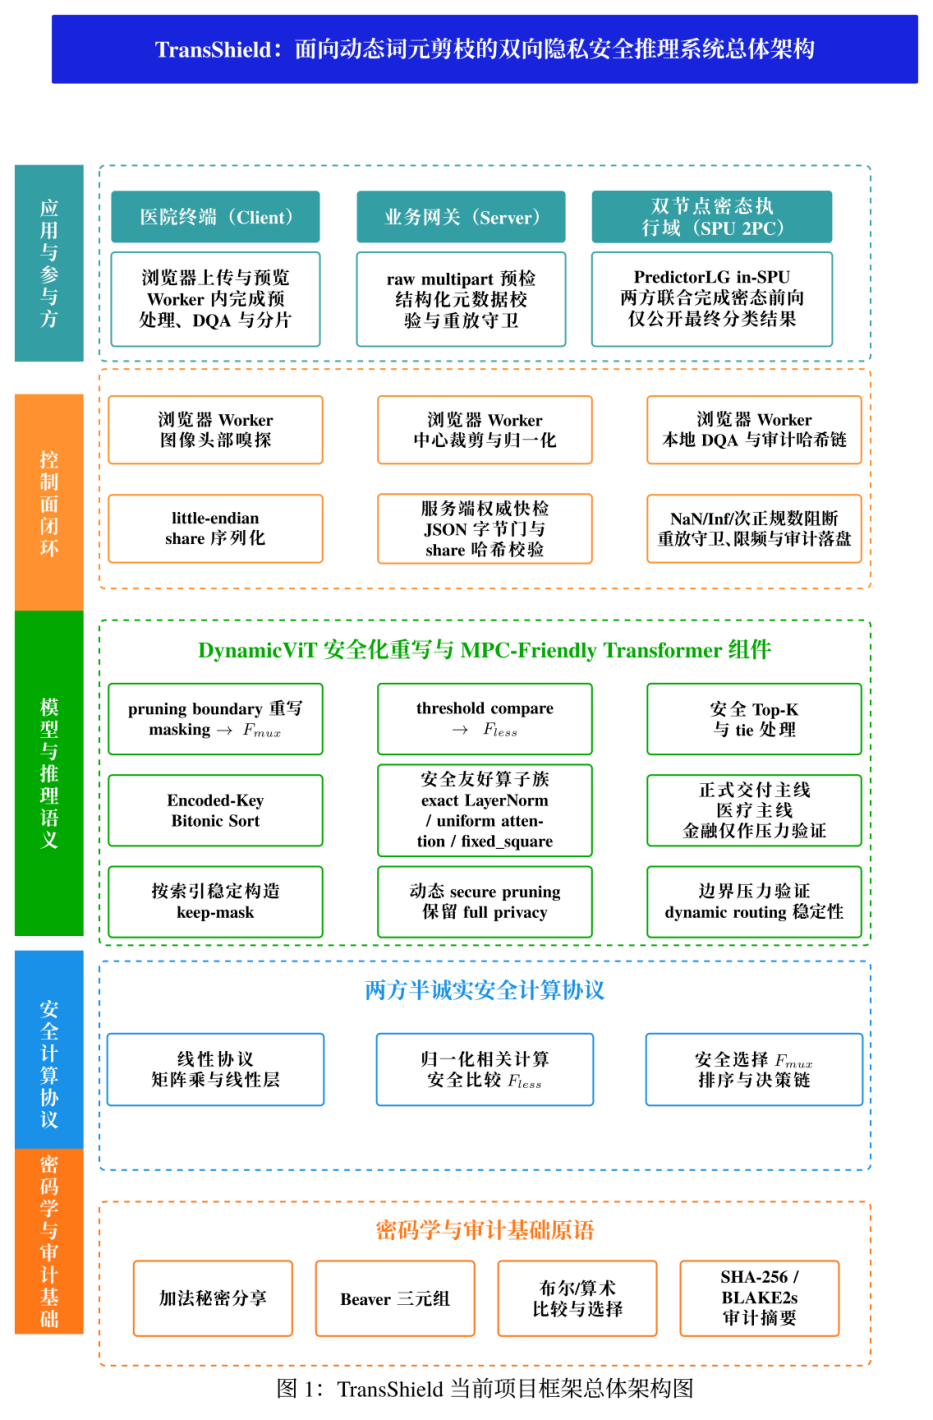
\includegraphics[width=0.92\textwidth]{figures/fig3-1-project-architecture.png}
\caption{图3-1 密捷项目当前框架总体架构图。}
\end{figure}

图3-1可按“终端本地明文处理—跨域密态传输—服务端入口门控—双节点密态执行—结果回传与审计固化”五个层次理解。图左侧的医院终端代表数据提供方，也是整条链路中唯一允许接触原始影像、明文像素张量和局部质量指标的位置；图右侧的双节点密态执行域代表模型持有方与协同计算方在两方半诚实安全计算约束下共同完成推理的区域；两者之间由业务网关和服务端控制面构成一道明确的信任边界。

从输入侧开始，用户在浏览器端选择影像后，主线程并不直接承担高开销计算，而只负责文件句柄保留、界面状态维护与请求编排。真正的图像头部尺寸检查、异常尺寸阻断、解码、中心裁剪、像素归一化、本地数据质量评估、审计哈希链构建以及 share0/share1 的小端序 Float32 序列化，全部在浏览器工作线程内部完成。换言之，图3-1中“医院终端”内部已经同时完成了明文处理、质量预检与秘密分享三项职责，这是原始像素不越出终端侧的关键。

当终端侧形成两份密态分片与结构化元数据后，跨越信任边界传输的对象就被严格限制为：share 字节流、审计摘要和最小必要的结构化质量信息，而不是原始图像或可逆像素值。进入服务端后，业务网关首先负责请求体大小、boundary 参数、多部件结构和字段集合的快速预检；随后，权威快检模块继续完成 JSON 字节长度门、share 哈希校验、内存对齐复制、非有限数与次正规数阻断、张量幅值检查、质量摘要容差复核、nonce 重放拦截、payload 去重以及来源地址并发守卫。只有在这些门控全部通过后，请求才会被转送至下游 SPU 密态执行域。

图3-1中部的 DynamicViT 安全化重写组件用于说明：本作品并不是把一个静态模型简单包进安全计算框架，而是对动态词元剪枝路径本身做了协议友好改写。具体而言，PredictorLG 在 SPU 内部生成词元得分，编码键排序网络在固定图中完成稳定的保留边界推导与 keep-mask 构造，后续 attention、MLP、残差连接和分类头始终保持在两方安全执行域内运行。这样既保留了按样本变化的动态剪枝能力，又避免把剪枝决策暴露为外部明文控制流，从而使“动态”与“密态”真正统一到同一条执行链路中。

在输出侧，SPU 域对外仅释放最终分类结论，而不会泄露中间特征、模型参数或任一方的明文 share。服务端控制面同时补充返回质量裁决、审计摘要与控制面耗时，并将关键事件写入审计记录，以便展示、复核与赛后核查使用同一条证据链。因此，图3-1不仅展示了系统由哪些模块构成，更重要的是交代了每一类数据在什么位置生成、在什么边界停止、由谁执行校验，以及最终以何种最小暴露形式返回结果；沿着这条责任链阅读，即可完整理解本作品从上传、门控、推理到审计的整体运作流程。

与固定结构 Transformer 私有推理路线相比，本作品在模型改造阶段优先解决的是“动态决策链如何留在安全执行域内”。Iron[18]、BOLT[19]、BumbleBee[7] 和 NEXUS[20] 主要围绕固定结构模型的矩阵乘、Softmax、LayerNorm、GELU 或交互轮次进行协议级优化；而本作品首先保留视觉 DynamicViT 的逐 stage 保留语义，再把删除式剪枝重写为 keep-mask 驱动的固定图执行。这一差异决定了本作品的贡献重点不在于单独压缩某个算子，而在于让动态词元剪枝本身能够在两方安全执行链路中稳定落地。

\section{端到端执行流程与模块协同}

结合图 3-1 的当前项目框架，当前端到端链路可以压缩为三个安全阶段。第一阶段是终端本地预处理：浏览器工作线程完成影像解码、质量评估、审计链构建与秘密分享，安全目标是使原始影像和明文像素止于终端侧。第二阶段是服务端边界拦截：前置网关与权威快检模块在进入 SPU 之前完成报文、结构化元数据、share 字节流与重构张量合法性校验，安全目标是使异常输入、重放请求和畸形张量止于密态执行入口之外。第三阶段是 SPU 密态执行：PredictorLG、编码键排序、keep-mask 构造与前向分类全部保留在两方安全执行域内，安全目标是避免动态决策链退化为外部明文回放。

因此，本节不再重复图 2-2 中的逐步动作，而是强调各阶段的安全职责分工：前端负责明文边界与分片生成，服务端负责权威阻断与审计固化，SPU 路径负责完成双向隐私约束下的动态安全推理。

\section{前端控制面实现}

前端实现采用主线程与单实例浏览器工作线程分离的结构。主线程只负责文件句柄保留、页面状态维护和请求编排；工作线程内部完成图像头部尺寸嗅探、异常尺寸阻断、解码与中心裁剪、数据质量指标提取、源图与 share 审计哈希计算、小端序 32 位浮点（Float32）字节流序列化与可转移数组缓冲区传递。该设计避免了大体量数组在主线程上的结构化克隆开销，同时将高开销计算与页面交互解耦。

前端计算过程中的关键数值变换、两方分片关系与审计关系见式（3-3）至式（3-5），其中式（3-4a）进一步给出输入张量与两方 share 之间的对应关系：

\begin{equation}
x_{c,h,w}=\operatorname{clip}\!\left(\frac{\frac{p_{c,h,w}}{255}-\mu_c}{\sigma_c},-2,2\right)
\tag{3-3}
\end{equation}

\begin{equation}
\operatorname{share0}_{c,h,w}=r_{c,h,w}, \quad r_{c,h,w}\sim U[-2,2], \quad \operatorname{share1}_{c,h,w}=x_{c,h,w}-\operatorname{share0}_{c,h,w}
\tag{3-4}
\end{equation}

\begin{equation}
x_{c,h,w}=\langle x_{c,h,w}\rangle_{0}+\langle x_{c,h,w}\rangle_{1}, \quad \langle x_{c,h,w}\rangle_{0}=\operatorname{share0}_{c,h,w}, \quad \langle x_{c,h,w}\rangle_{1}=\operatorname{share1}_{c,h,w}
\tag{3-4a}
\end{equation}

\begin{equation}
H_{\text{audit}}=\operatorname{SHA256}\!\left(v7 \parallel nonce \parallel H(src) \parallel H(x) \parallel H(\operatorname{share0}) \parallel H(\operatorname{share1})\right)
\tag{3-5}
\end{equation}

其中，$p_{c,h,w}$ 表示裁剪后图像在通道 $c$、位置 $(h,w)$ 的原始像素值，$\mu_c$ 与 $\sigma_c$ 分别对应 ImageNet 均值与标准差，$x_{c,h,w}$ 为送入模型的归一化张量值；式（3-4a）中的 $\langle x_{c,h,w}\rangle_0$ 与 $\langle x_{c,h,w}\rangle_1$ 对应浏览器端生成的两份 additively split share，并在传输层分别落到 share0 与 share1。为避免浏览器端异常数值写入底层缓冲区，前端会先将归一化结果裁剪到 [-2, 2]，再以 little-endian Float32 方式写入 share 字节流；审计链则把源图哈希、归一化张量哈希与两份 share 哈希绑定到同一个 nonce 上。

为便于直观看清主线程与浏览器工作线程的职责边界，图 3-2 将文件句柄保留、页面状态维护、可转移数组缓冲区传递、图像预处理、审计哈希与秘密分享生成拆解为三个协同区域。该图对应本节实现要点：主线程只负责交互与调度，工作线程承担高开销计算，并在跨越信任边界前完成明文终止与密态分片生成。

\begin{figure}[htbp]
\centering
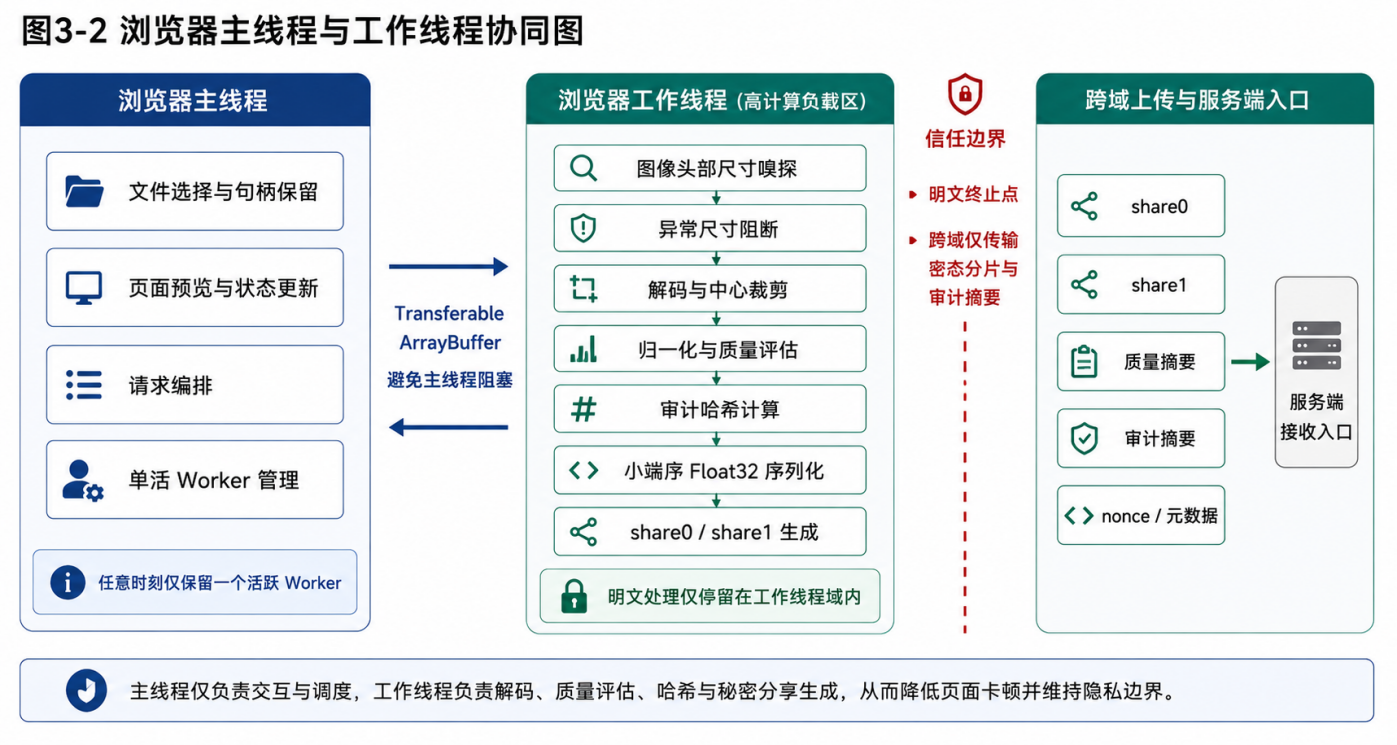
\includegraphics[width=0.92\textwidth]{figures/fig3-2-browser-worker-collaboration.png}
\caption{图3-2 浏览器主线程与工作线程协同图：主线程负责交互与调度，工作线程负责预处理、哈希与秘密分享生成。}
\end{figure}

\section{服务端权威快检与审计}

服务端在进入 SPU 之前，依次执行原始报文体读取上限、boundary 参数解析、多部件表单（multipart）原始结构预检、精确字段集约束、单字段 JSON 字节长度门、严格 UTF-8 结构化元数据解析、share 哈希校验、张量重构前内存对齐复制、非有限数与次正规数阻断、服务端数据质量复核，以及 nonce、payload 与来源 IP 维度的重放与并发守卫。审计层同时记录哈希摘要、控制面开销与事件落盘结果，以保证前端展示、服务端阻断与事后核查使用的是同一条证据链。

服务端快检并非只核对客户端声明，而是围绕重构张量、质量摘要与容差关系进行权威复算。关键关系见式（3-6）至式（3-9b），其中式（3-6a）给出最终分类输出的恢复关系：

\begin{equation}
X=\operatorname{share0}+\operatorname{share1}, \quad RGB=X\odot \sigma+\mu
\tag{3-6}
\end{equation}

\begin{equation}
z_c=\langle z_c\rangle_{0}+\langle z_c\rangle_{1}, \quad \hat{y}=\arg\max_c z_c
\tag{3-6a}
\end{equation}

\begin{equation}
L_i=0.299R_i+0.587G_i+0.114B_i, \quad \operatorname{OverExp}=\frac{1}{N}\sum_{i=1}^{N}\mathbf{1}\!\left[L_i\ge 0.95\right]
\tag{3-7}
\end{equation}

\begin{equation}
\operatorname{lap}(x,y)= -4L(x,y)+L(x-1,y)+L(x+1,y)+L(x,y-1)+L(x,y+1)
\tag{3-8}
\end{equation}

\begin{equation}
\Delta_k=\left|q_k^{(\text{client})}-q_k^{(\text{server})}\right|, \quad \Delta_k \le 10^{-4}
\tag{3-9}
\end{equation}

\begin{equation}
\mu_{\text{lap}}=\frac{1}{HW}\sum_{x=1}^{H}\sum_{y=1}^{W}\operatorname{lap}(x,y), \quad \sigma_{\text{lap}}^{2}=\frac{1}{HW}\sum_{x=1}^{H}\sum_{y=1}^{W}\left(\operatorname{lap}(x,y)-\mu_{\text{lap}}\right)^{2}
\tag{3-8a}
\end{equation}

\begin{equation}
F_{\text{payload}}=\operatorname{BLAKE2s}\!\left(H(\operatorname{share0}) \parallel \text{:} \parallel H(\operatorname{share1})\right)
\tag{3-9a}
\end{equation}

\begin{equation}
n_{\text{ip}}(t;\Delta)=\sum_j \mathbf{1}\!\left[t-\Delta \le t_j \le t\right], \quad n_{\text{ip}}(t;\Delta)\le R_{\text{ip}}, \quad c_{\text{ip}}^{\text{inflight}}\le C_{\text{ip}}
\tag{3-9b}
\end{equation}

式（3-6a）给出最终类别 logit 的两方恢复关系；式（3-8a）将离散拉普拉斯响应进一步归约为方差指标，用于度量局部纹理与边缘强度；式（3-9a）与式（3-9b）分别对应载荷指纹去重与来源地址限频 / 并发守卫，从而把服务端控制面中的“去重、限频、准入”逻辑形式化为可验证约束。

其中，服务端会先对 share 执行内存对齐复制，再将绝对值小于 $2^{-126}$ 的极小值刷新为零，以切断次正规数带来的微代码异常路径；随后检查 share 与重构张量是否存在非有限值，以及 share 幅值是否超过 $2$。对客户端与服务端分别得到的质量摘要 $q_k^{(\text{client})}$ 与 $q_k^{(\text{server})}$，只在基础连续数值出现显著偏离时才标记可疑漂移，而不会仅凭离散风险标签不一致就直接判定篡改。

为了把服务端权威快检、重放防护、并发守卫与审计落盘过程概括为可执行步骤，算法3给出服务器侧的统一验证与审计流程。

为便于对应服务端控制面的实际落地点，图 3-3 将权威快检与审计闭环拆解为原始请求体读取、协议结构预检、JSON 长度门、share 哈希校验、张量快检、重放并发守卫与审计落盘等连续门控步骤。该图与本节公式部分共同说明：客户端声明不会直接成为最终裁决依据，请求只有在全部检查通过后才会进入 SPU 密态执行域。

本章出现的核心数学符号及其含义汇总如表 5 所示。

\begin{figure}[htbp]
\centering
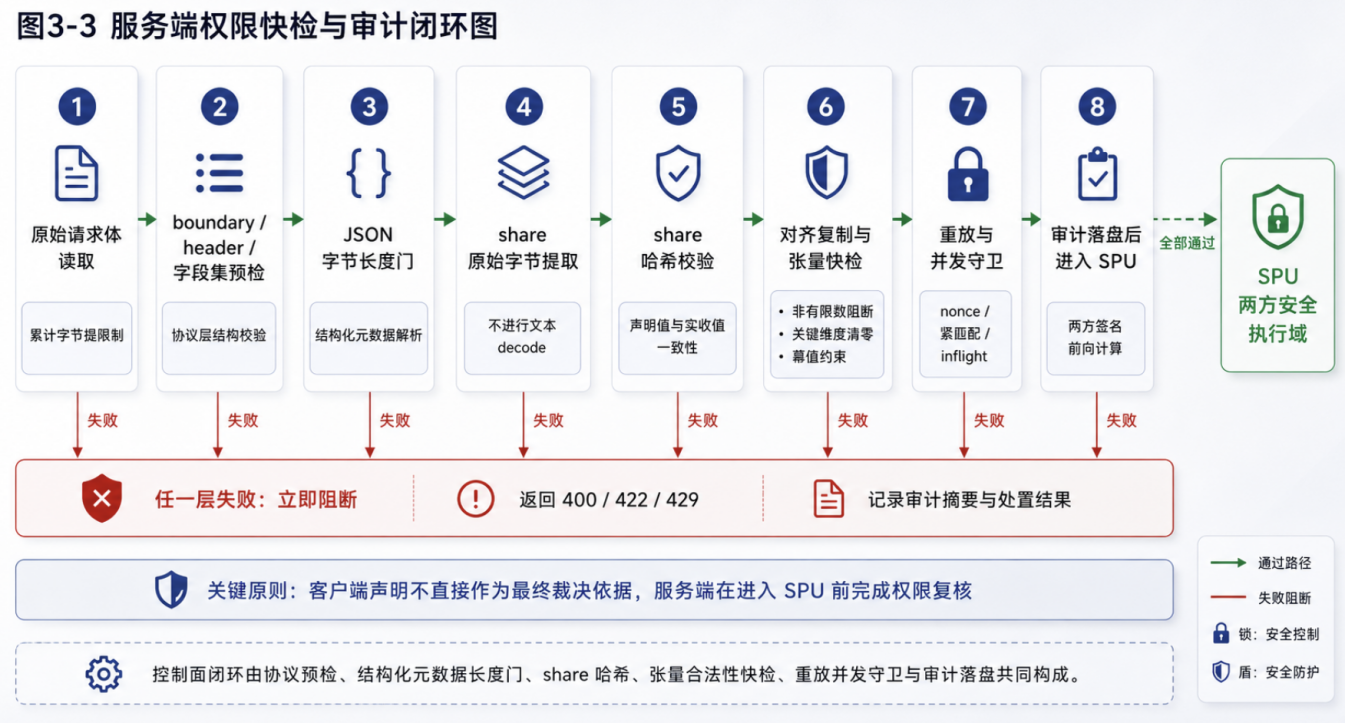
\includegraphics[width=0.92\textwidth]{figures/fig3-3-control-plane-gates.jpeg}
\caption{图3-3 服务端权威快检与审计闭环图：请求仅在全部门控通过后进入 SPU，任一层失败均立即阻断并记录审计结果。}
\end{figure}

\begin{longtable}{>{\raggedright\arraybackslash}p{0.32\textwidth}>{\raggedright\arraybackslash}p{0.32\textwidth}>{\raggedright\arraybackslash}p{0.32\textwidth}}
\caption{表 5 第三章关键符号说明}\\
\toprule
\textbf{符号} & \textbf{含义} & \textbf{出现位置} \\
\midrule
\endfirsthead
\toprule
\textbf{符号} & \textbf{含义} & \textbf{出现位置} \\
\midrule
\endhead
 & 第 l 个剪枝 stage 的词元得分向量 & 式(3-1) \\
 & 第 l 个剪枝 stage 允许保留的词元数 & 式(3-1) \\
 & 由安全 Top-边界导出的保留阈值 & 式(3-1) \\
 & 编码键与经双调排序得到的索引排列 & 式(3-2a)、式(3-2b) \\
 & 第 i 个词元在第 l 个 stage 的保留掩码 & 式(3-1)、式(3-2)、式(3-2b) \\
 & 原始词元表征与掩码后的词元表征 & 式(3-2) \\
 & 裁剪后图像在通道 c、位置 (h,w) 的原始像素值 & 式(3-3) \\
 & 通道 c 的归一化均值与标准差 & 式(3-3)、式(3-6) \\
 & 归一化后的模型输入张量 & 式(3-3)、式(3-4) \\
 & 针对输入张量构造的两份秘密分享分片 & 式(3-4) \\
 & 第 k 个质量指标及其客户端/服务端绝对偏差 & 式(3-9) \\
 & 像素总数、亮度值与离散拉普拉斯响应 & 式(3-7)、式(3-8) \\
\bottomrule
\end{longtable}

\section{关键交付物与证据落点}

本作品的核心交付物、仓内存储路径与用途说明如表 6 所示。

工程实现上，模型部署包不仅包含权重和推理参数，还包含用于解释执行边界的 manifest 信息。该信息用于约束输入形状、剪枝阶段、保留比例、近似算子配置和审计字段，使训练导出的模型语义、SPU 执行闭包和前端展示内容能够相互校验。这样做可以降低“模型已更新但展示仍引用旧指标”或“配置变更后安全边界描述失真”的风险，也使报告中的实验指标能够回溯到仓内实际文件。

\begin{longtable}{>{\raggedright\arraybackslash}p{0.32\textwidth}>{\raggedright\arraybackslash}p{0.32\textwidth}>{\raggedright\arraybackslash}p{0.32\textwidth}}
\caption{表 6 系统关键交付物与仓内落点说明}\\
\toprule
\textbf{类别} & \textbf{仓内落点} & \textbf{用途} \\
\midrule
\endfirsthead
\toprule
\textbf{类别} & \textbf{仓内落点} & \textbf{用途} \\
\midrule
\endhead
前后端演示程序 & showcase/src/；showcase/src/workers/medicalControlPlaneWorker.ts；showcase\_api/app.py；showcase\_api/control\_plane.py & 承载浏览器工作线程、服务端权威快检、页面交互与 /api/medical/live-run 入口 \\
自动化验证脚本 & tools/showcase\_protocol\_fuzz.py；tools/showcase\_guard\_stress.py & 验证协议层异常输入、重放与并发守卫 \\
图件与报告生成脚本 & tools/showcase\_extract\_report\_assets.py；showcase/public/report-assets/；showcase/src/generated/report\_content.json & 从正式 DOCX 提取展示图件与章节 JSON，用于重建展示站内容 \\
复现说明 & README\_REPRODUCE.md & 提供环境约束、运行步骤与预期输出 \\
许可证与修改映射 & spu\_vendored/LICENSE；spu\_vendored/MODIFICATIONS.md；THIRD\_PARTY.md & 支撑第三方许可与本地修改说明 \\
\bottomrule
\end{longtable}

\noindent\textit{注：所有交付物均已纳入版本控制，仓内路径与本表格完全一致；自动化验证脚本可直接运行生成对应证据文件。}


\chapter{测试方案与结果分析}
\section{测试环境、数据与评价指标}

本次测试使用的数据集规模、用途与核心评价指标如表 7 所示。实验主要使用 524 张验证集样本进行医疗主线评估，另使用 8 条金融边界压力样本进行迁移性与稳定性验证。医疗主线采用阈值精度、AUC 和 argmax 精度作为主要指标，其中阈值精度用于反映部署口径下的最终分类效果，AUC 用于衡量整体判别能力，argmax 精度用于描述未校准条件下的直接决策表现。协议层与控制面验证则采用异常输入拦截率、重放拦截率、并发守卫结果和审计落盘状态作为主要观察指标。

需要说明的是，本文中涉及的性能结果均以固定 checkpoint 和同口径验证集为基础，反映的是部署态结果而非多随机种子的训练均值。

\begin{longtable}{>{\raggedright\arraybackslash}p{0.24\textwidth}>{\raggedright\arraybackslash}p{0.24\textwidth}>{\raggedright\arraybackslash}p{0.24\textwidth}>{\raggedright\arraybackslash}p{0.24\textwidth}}
\caption{表 7 测试数据集与评价指标说明}\\
\toprule
\textbf{对象} & \textbf{样本规模} & \textbf{作用} & \textbf{主要指标} \\
\midrule
\endfirsthead
\toprule
\textbf{对象} & \textbf{样本规模} & \textbf{作用} & \textbf{主要指标} \\
\midrule
\endhead
医疗全量验证集 & 524 张 & 正式阈值搜索与精度评估 & argmax 精度、阈值精度、部署阈值 \\
医疗部署验证批次 & 32 张 & 完整双向隐私原型运行 & 平均时延、双向总通信量、隐私边界 \\
金融边界压力样本 & 8 条 & 极端分布输入下的稳定性验证 & 逐样本一致性、时延、通信量 \\
协议层与控制面黑盒用例 & 17 类 & 异常输入、重放与并发探针验证 & 首个拦截层、兜底层级、资源状态 \\
\bottomrule
\end{longtable}

\section{基线对比}

\begin{figure}[htbp]
\centering
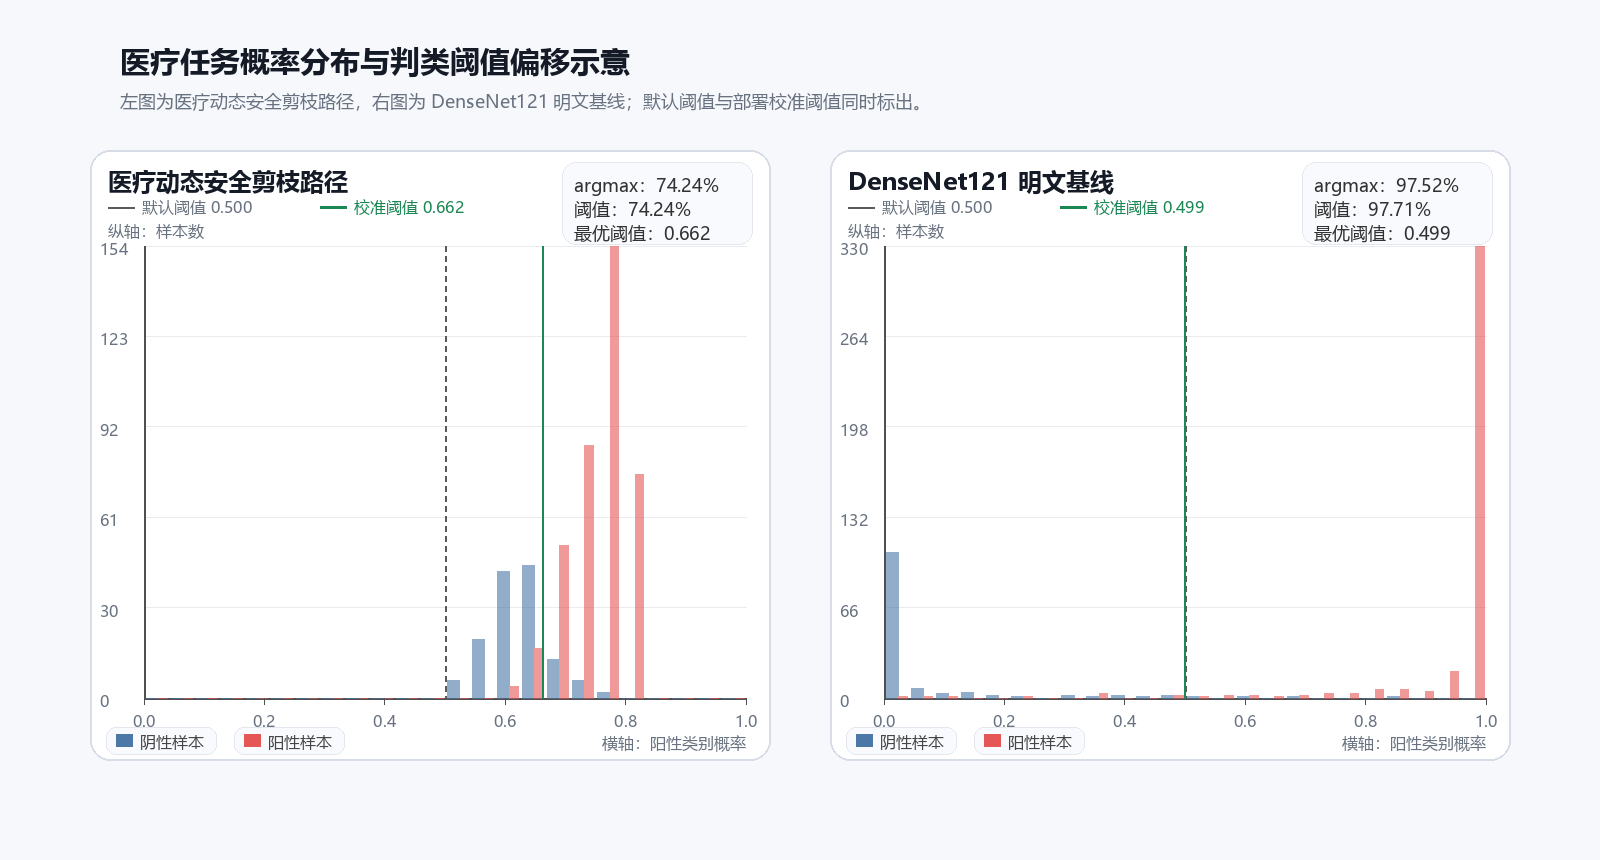
\includegraphics[width=0.92\textwidth]{figures/fig4-1-threshold-shift.png}
\caption{图4-1 不同方案医疗任务性能基线对比}
\end{figure}

本作品与不同基线方案在医疗任务上的性能对比结果如图4-1 所示。从同仓与外部对比结果看，本作品医疗动态安全剪枝链路相较固定结构静态对照线提升 0.7634 个百分点，相较当前仓内可复现的原始 DynamicViT 基线提升 17.3664 个百分点，说明协议友好重写并未使动态路径退化为不可部署状态。另一方面，与同数据集强明文参考 MPCViT（面向多方计算的视觉 Transformer）相比，本作品当前仍存在 4.2366 个百分点的阈值精度差距；与同架构静态上界 DeiT-S（数据高效图像 Transformer 小型模型）相比，差距为 3.2419 个百分点。这些差距说明本作品的价值主要在于“双向隐私 + 动态剪枝安全执行”的系统能力，而不是在明文精度指标上全面超过所有强明文参考。

需要说明的是，外部对比表中“原始 DynamicViT”一行现统一采用当前仓内与服务器均可复现的原始明文基线口径。此前遗留的“20 epoch / 80.73\%”旧值未能在最终交付仓与服务器环境中追溯到配套权重文件，因此本次修订不再继续引用该旧数值。

\section{医疗主要交付场景结果}

\begin{longtable}{>{\raggedright\arraybackslash}p{0.32\textwidth}>{\raggedright\arraybackslash}p{0.32\textwidth}>{\raggedright\arraybackslash}p{0.32\textwidth}}
\caption{表 8 医疗主要交付场景核心指标结果}\\
\toprule
\textbf{指标} & \textbf{结果} & \textbf{说明} \\
\midrule
\endfirsthead
\toprule
\textbf{指标} & \textbf{结果} & \textbf{说明} \\
\midrule
\endhead
全量验证集 argmax 精度 & 74.2366\% & 反映动态路径在默认决策边界下的直接分类结果 \\
全量验证集阈值精度 & 92.7481\% & 基于 524 张验证样本完成统一阈值搜索后的正式指标 \\
全量验证集 AUC & 0.9639 & 2026 年 5 月 20 日服务器按同口径重跑补齐 \\
部署阈值 & 0.6619606018 & 动态路径单独校准后的正式部署阈值 \\
32 条样本验证批次平均时延 & 89.06 秒/样本 & 当前主要交付场景的端到端双向隐私原型口径 \\
32 条样本验证批次双向通信量 & 84.47 GiB & 来自同配置重测记录的双向通信总量 \\
隐私边界 & 服务端不接收明文像素值，模型参数不以明文暴露 & 对外仅返回最终分类结果 \\
\bottomrule
\end{longtable}

医疗主要交付场景下的核心精度、性能与隐私边界指标如表 8 所示。图 4-2 对比了医疗动态安全剪枝路径与 DenseNet121 明文卷积基线的概率分布及阈值位置。结合 argmax 精度与阈值精度可以看出，当前动态路径的主要问题并非样本排序能力完全丧失，而是部署边界相对固定结构参考发生了系统性偏移。因此，针对动态路径单独校准部署阈值，是当前交付方案中的必要步骤。

\begin{figure}[htbp]
\centering
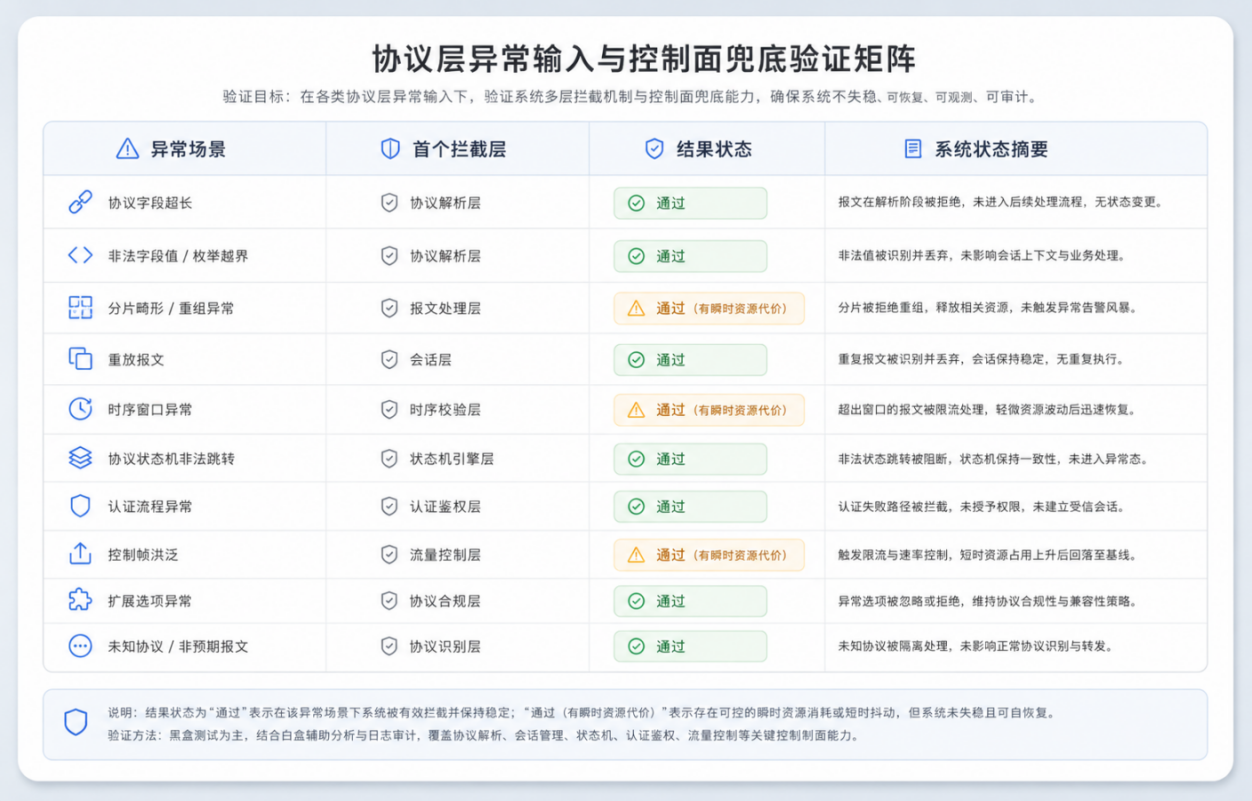
\includegraphics[width=0.92\textwidth]{figures/fig4-2-guard-matrix.png}
\caption{图4-2 医疗动态安全剪枝路径与 DenseNet121 明文基线的概率分布与阈值偏移对比。}
\end{figure}

同口径服务器复核表明，医疗动态安全剪枝链路在 full-val CPU runtime-pruning reference 口径下的 AUC 为 0.9639。这说明当前动态路径并未失去样本排序能力，影响部署效果的关键问题仍然是决策边界相对固定结构参考发生系统性偏移，因此动态路径单独阈值校准仍是正式部署中的必要步骤。

\section{性能与通信量分析}

医疗交付场景与金融边界压力验证场景的端到端性能与通信量统计结果如图4-3所示。

\reportmissingfigure{4-3}{图4-3 不同场景端到端性能与通信量统计}

\noindent\textit{注：通信量为两方节点之间的双向总字节数，包含协议头与控制报文；所有测试均在同机本地双节点（colocated localhost）2PC 模式下执行。}

为进一步量化算子优化的收益，本作品补充了统一基准下的算子级代理对比，结果如表9所示。

\begin{longtable}{>{\raggedright\arraybackslash}p{0.24\textwidth}>{\raggedright\arraybackslash}p{0.24\textwidth}>{\raggedright\arraybackslash}p{0.24\textwidth}>{\raggedright\arraybackslash}p{0.24\textwidth}}
\caption{表 9 算子级代理基准对比结果}\\
\toprule
\textbf{代理基准对比组} & \textbf{通信比值 （左/右）} & \textbf{时间比值 （左/右）} & \textbf{适用范围说明} \\
\midrule
\endfirsthead
\toprule
\textbf{代理基准对比组} & \textbf{通信比值 （左/右）} & \textbf{时间比值 （左/右）} & \textbf{适用范围说明} \\
\midrule
\endhead
同形状算子代理基准 & 0.149x & 0.528x & 同一模型形状、同一 2PC benchmark harness；主要用于观察算子配置导致的安全开销差异。 \\
异构结构代理基准 & 16.845x & 2.955x & 同一 MPCFormer local 2PC benchmark harness；各 profile 使用各自模型结构参数。这不是 full-val 医学图像 pipeline 通信量。 \\
\bottomrule
\end{longtable}

\noindent\textit{注："同形状算子代理基准" 基于统一 DeiT-S 模型结构测试；"异构结构代理基准" 仅用于说明模型结构差异对性能的影响，不代表医疗端到端链路性能。}

为便于统一表达时延与通信量的来源，本节先用式（4-1）至式（4-2）给出端到端代价的分解形式，再结合当前原型链路的实测结果解释主要瓶颈。

\begin{equation}
T_{\text{total}}=T_{\text{pre}}+T_{\text{guard}}+T_{\text{SPU}}+T_{\text{post}}
\tag{4-1}
\end{equation}

\begin{equation}
V_{\text{total}}=\sum_{r}\left(V_{\text{send}}^{r}+V_{\text{recv}}^{r}\right), \quad \rho_V=\frac{V_{\mathrm{Transshield}}}{V_{\text{ref}}}, \quad \rho_T=\frac{T_{\mathrm{Transshield}}}{T_{\text{ref}}}
\tag{4-2}
\end{equation}

其中，$T_{\text{total}}$ 由前端预处理、服务端控制面快检、SPU 密态执行与结果回传/审计收尾四部分组成；$V_{\text{total}}$ 表示一次完整推理的双向总通信量，$\rho_V$ 与 $\rho_T$ 分别表示相对通信量与相对时延比。

性能证据分为两层：其一是上述端到端双向隐私运行结果，用于说明医疗动态安全剪枝链路与金融压力样本在当前原型中的总时延和总通信量；其二是统一安全基准下的算子级代理对比，用于说明算子替换本身的开销趋势。在固定同一 DeiT-S 形状的代理基准对比中，密捷的安全友好算子将通信压缩到外部基准算子的 0.149 倍，时间压缩到 0.528 倍，说明算子替换本身具有正向收益。另一方面，跨模型结构的异构结构代理基准只能用于说明结构尺度差异会显著放大绝对代价，不能与医疗全量验证链路混写。

当前时延与通信量偏高，主要由三类因素共同造成。第一，动态安全剪枝链路保留了词元剪枝的密态比较、排序与掩码化决策链，相比固定结构安全推理会引入额外的协议轮次。第二，当前运行口径是同机本地双节点（colocated localhost）2PC 原型链路，虽然两方节点位于同一服务器内，但张量交换、线性层通信与 softmax 归一化指数函数相关算子仍构成主要代价来源，不能将 localhost 原型误解为“几乎无通信成本”。第三，当前 Web 演示后端以正确性与边界防护为首要目标，未针对生产级吞吐做异步化、流水化或任务队列改造。因此，本报告只保留已直接落盘的端到端结果与算子级代理证据，不额外给出未经观测的阶段占比、P50/P95 延迟或生产级并发吞吐承诺。

\section{金融边界压力验证结果}

金融边界压力验证场景下的核心指标结果如表 10 所示。需要说明的是，金融域原始输入并非自然图像，而是信用卡欺诈检测任务中的 30 维 PCA 特征。为了复用 DeiT-S 的块嵌入（Patch Embedding）结构，本作品先将一维金融特征通过拟图像空间连续性编码映射为 224×224 灰度图，使输入保留可供视觉 Transformer 利用的局部平滑先验。仓内冻结 bundle 记录表明，早期的 patch-based 与 DCT 编码未形成稳定可用结果，当前边界压力验证对应的是 v3 image-like smooth/contrast encoding。

\begin{longtable}{>{\raggedright\arraybackslash}p{0.32\textwidth}>{\raggedright\arraybackslash}p{0.32\textwidth}>{\raggedright\arraybackslash}p{0.32\textwidth}}
\caption{表 10 金融边界压力验证核心指标}\\
\toprule
\textbf{指标} & \textbf{结果} & \textbf{说明} \\
\midrule
\endfirsthead
\toprule
\textbf{指标} & \textbf{结果} & \textbf{说明} \\
\midrule
\endhead
8 条压力样本逐样本一致性 & 8 / 8 样本差异为 0 & 与明文参考逐样本对齐 \\
部署效率 & 106.16 秒/样本 & 仅作为边界压力验证口径 \\
双向总通信量 & 25.30 GiB & 同配置重测口径 \\
参数规模保留比例 & 68.39\% & 体现低秩压缩收益 \\
\bottomrule
\end{longtable}

金融部分仅承担方法迁移性与极端输入稳定性验证职责，不作为与医疗并列的独立交付场景。其价值在于：在不改变安全运行链基本结构的前提下，验证控制面、动态路由与安全执行语义在另一类高敏感任务中的边界表现，从而证明本作品的工程设计并非只对单一数据分布有效。

\section{协议层异常输入与鲁棒性验证}

鲁棒性验证采用穷举边缘分支矩阵，而不是以单一拦截率概括系统表现。协议层测试覆盖分块传输编码（Transfer-Encoding: chunked）、超大报文长度声明（Content-Length）、boundary 参数混淆、重复字段、畸形分片报文头、空字节注入、非空尾部附加数据、UTF-16 编码结构化元数据、超长结构化元数据以及截断请求体；控制面测试覆盖随机一次性标识（Nonce）并发重放、相同载荷更换 Nonce、同一来源地址并发占满与短窗限频。每个用例均记录首个拦截层、兜底层级、返回处置与资源状态回落摘要，以同时证明拦截有效性与系统可服务性。协议层与控制面鲁棒性验证的整体统计结果如表 11 所示。

\begin{longtable}{>{\raggedright\arraybackslash}p{0.16\textwidth}>{\raggedright\arraybackslash}p{0.16\textwidth}>{\raggedright\arraybackslash}p{0.16\textwidth}>{\raggedright\arraybackslash}p{0.16\textwidth}>{\raggedright\arraybackslash}p{0.16\textwidth}>{\raggedright\arraybackslash}p{0.16\textwidth}}
\caption{表 11 协议层与控制面鲁棒性验证统计}\\
\toprule
\textbf{测试组} & \textbf{用例数} & \textbf{按预期通过} & \textbf{FD/Socket无泄漏} & \textbf{稳态回落用例} & \textbf{证据文件} \\
\midrule
\endfirsthead
\toprule
\textbf{测试组} & \textbf{用例数} & \textbf{按预期通过} & \textbf{FD/Socket无泄漏} & \textbf{稳态回落用例} & \textbf{证据文件} \\
\midrule
\endhead
协议层异常输入 & 13 & 13 / 13 & 13 / 13 & 11 / 13 & 协议异常输入验证记录 \\
控制面守卫 & 4 & 4 / 4 & 4 / 4 & 1 / 4 & 控制面守卫验证记录 \\
合计 & 17 & 17 / 17 & 17 / 17 & 12 / 17 & 汇总 \\
\bottomrule
\end{longtable}

从当前留存结果看，协议层异常输入与控制面守卫共覆盖 17 类黑盒用例，17/17 均返回预期拦截或限制结果；全部用例在采样窗口内均未观察到文件描述符或套接字文件描述符的净增长。与此同时，部分并发与大负载探针会带来瞬时常驻内存抬升，因此本作品将其如实记录为“资源成本存在但句柄未泄漏”，而不是将其包装为零成本防护。

为适配 A4 版面，鲁棒性验证矩阵拆分为两张窄表：前表记录攻击特征与拦截链，后表记录返回处置、资源状态与证据来源；为便于对照阅读，第二张表重复给出“异常场景”列。其中，表示文件描述符数量变化，表示套接字文件描述符数量变化，表示常驻内存变化，表示线程数变化，四项指标均按异常处理后观测值减去基线观测值计算。各类异常场景的攻击特征与系统拦截层级明细如表 12 所示。对应异常场景的系统返回处置、资源状态与证据来源明细如表13所示

\begin{longtable}{>{\raggedright\arraybackslash}p{0.24\textwidth}>{\raggedright\arraybackslash}p{0.24\textwidth}>{\raggedright\arraybackslash}p{0.24\textwidth}>{\raggedright\arraybackslash}p{0.24\textwidth}}
\caption{表 12 异常场景攻击特征与拦截层级明细（上）}\\
\toprule
\textbf{异常场景} & \textbf{攻击载荷特征} & \textbf{首个拦截层级} & \textbf{兜底层级} \\
\midrule
\endfirsthead
\toprule
\textbf{异常场景} & \textbf{攻击载荷特征} & \textbf{首个拦截层级} & \textbf{兜底层级} \\
\midrule
\endhead
Chunked 编码绕过 & Transfer-Encoding: chunked，绕过 Content-Length & HTTP 请求体入口门 & 不适用 \\
超大 Content-Length & 声明体积超过 5 MiB，验证 413 + 强制阻断 & Content-Length 头部上限门 & TCP 强制阻断兜底 \\
重复字段名 & 重复注入 multipart 字段，诱导字段集歧义 & raw multipart 预检 & MIME 结构校验 \\
Boundary 扇出 & 构造过多分片，放大 MIME 解析树 & raw multipart 预检 & MIME 结构校验 \\
嵌套 multipart & 把 share part 伪装成 multipart/mixed & raw multipart 预检 & MIME 结构校验 \\
超长 JSON & client\_quality\_summary 超过 JSON 字节门 & JSON 字节长度门 & 严格 JSON 解码钩子 \\
字段集漂移 & 追加未声明字段，验证精确字段集约束 & raw multipart 预检 & 精确字段集门 \\
Boundary 参数混淆 & boundary 带空白与引号变体 & Content-Type boundary 解析 & raw multipart 预检 \\
畸形 Part Header & 缺失合法头格式，验证 header parser & multipart header 解析 & MIME 结构校验 \\
Header 空字节注入 & 在 part header 中注入 NUL / 控制字符 & multipart header 解析 & MIME 结构校验 \\
非空 Epilogue & closing boundary 后继续追加垃圾字节 & raw multipart 预检 & MIME 结构校验 \\
异常 JSON 字符集 & UTF-16LE 编码结构化元数据，验证严格 UTF-8 约束 & strict UTF-8 JSON 解码 & JSON 数值钩子 \\
截断请求体 & 提前断流，验证 streaming body reader & 流式 body 读取器 & 不适用 \\
重复 Nonce 并发重放 & 同 nonce 并发多发，验证幂等与重放防护 & Nonce 重放缓存门 & payload 指纹去重门 \\
同载荷换 Nonce & 相同 share 指纹 + 新 nonce，验证 payload 去重 & 载荷重放缓存门 & IP inflight 配额门 \\
同 IP 并发占满 & 单一来源地址并发冲击已通过前置校验的执行配额 & 单 IP inflight 守卫 & 全局 inflight 守卫 \\
短窗限频 & 同 IP 短时间空载请求探测限流门 & IP 滑动窗口限频 & 不适用 \\
\bottomrule
\end{longtable}

\begin{longtable}{>{\raggedright\arraybackslash}p{0.24\textwidth}>{\raggedright\arraybackslash}p{0.24\textwidth}>{\raggedright\arraybackslash}p{0.24\textwidth}>{\raggedright\arraybackslash}p{0.24\textwidth}}
\caption{表 13 异常场景返回处置与系统状态明细（下）}\\
\toprule
\textbf{异常场景} & \textbf{返回/处置} & \textbf{系统状态} & \textbf{证据来源} \\
\midrule
\endfirsthead
\toprule
\textbf{异常场景} & \textbf{返回/处置} & \textbf{系统状态} & \textbf{证据来源} \\
\midrule
\endhead
Chunked 编码绕过 & HTTP 400 / transfer\_encoding\_not\_supported & ；；KiB； & 协议异常输入验证记录 / A1 \\
超大 Content-Length & HTTP 413 / payload\_too\_large & ；；KiB； & 协议异常输入验证记录 / A2 \\
重复字段名 & HTTP 400 / malformed\_multipart\_precheck\_failed & ；；KiB； & 协议异常输入验证记录 / A3 \\
Boundary 扇出 & HTTP 400 / malformed\_multipart\_precheck\_failed & ；；KiB； & 协议异常输入验证记录 / A4 \\
嵌套 multipart & HTTP 400 / malformed\_multipart\_precheck\_failed & ；；KiB； & 协议异常输入验证记录 / A5 \\
超长 JSON & HTTP 400 / invalid\_control\_plane\_payload & ；；KiB； & 协议异常输入验证记录 / A6 \\
字段集漂移 & HTTP 400 / malformed\_multipart\_precheck\_failed & ；；KiB； & 协议异常输入验证记录 / A7 \\
Boundary 参数混淆 & HTTP 400 / malformed\_multipart\_precheck\_failed & ；；KiB； & 协议异常输入验证记录 / A8 \\
畸形 Part Header & HTTP 400 / malformed\_multipart\_precheck\_failed & ；；KiB； & 协议异常输入验证记录 / A9 \\
Header 空字节注入 & HTTP 400 / malformed\_multipart\_precheck\_failed & ；；KiB； & 协议异常输入验证记录 / A10 \\
非空 Epilogue & HTTP 400 / malformed\_multipart\_precheck\_failed & ；；KiB； & 协议异常输入验证记录 / A11 \\
异常 JSON 字符集 & HTTP 400 / invalid\_control\_plane\_payload & ；；KiB； & 协议异常输入验证记录 / A12 \\
截断请求体 & HTTP 400 / truncated\_body & ；；KiB； & 协议异常输入验证记录 / A13 \\
重复 Nonce 并发重放 & duplicate\_nonce×3；200×1 & ；；KiB； & 控制面守卫验证记录 / G1 \\
同载荷换 Nonce & 首发 200；复发 duplicate\_payload & ；；KiB； & 控制面守卫验证记录 / G2 \\
同 IP 并发占满 & 200×2；busy\_retry\_later×2 & ；；KiB； & 控制面守卫验证记录 / G3 \\
短窗限频 & invalid\_content\_length×6；rate\_limited\_ip×2 & ；；KiB； & 控制面守卫验证记录 / G4 \\
\bottomrule
\end{longtable}

\noindent\textit{注：系统状态指标 ΔFD、ΔSock、ΔRSS、ΔThr 均为异常处理完成后 10 秒的观测值与基线值的差值；所有证据文件均已留存于仓内 tools/evidence 目录。}

\reportmissingfigure{4-4}{图4-4 协议层异常输入与控制面兜底验证矩阵：同时显示首个拦截层级与文件描述符、套接字及常驻内存回落摘要。}

资源状态采用可观测代理指标描述，而不作无法直接证明的绝对化承诺。本文将“系统仍可服务”限定为：请求结束后 inflight 占用计数回落，文件描述符数量与套接字文件描述符数量回到基线附近，未观察到连接句柄持续泄漏；常驻内存在部分已通过前置校验的压力用例中出现瞬时抬升，但重复异常注入测试后未观察到单调持续增长，因此仅将其表述为原型阶段的瞬时资源成本，而不宣称所有指标完全归零。

\section{结果分析}

综合上述结果可以得到三个结论。第一，本作品动态安全剪枝链路的主要收益并非体现在超越强明文参考，而是体现在双向隐私约束下保留了可部署的动态剪枝能力，并通过阈值校准把全量验证集精度恢复到 92.7481\%。第二，算子级代理对比说明安全友好算子本身具有明显的通信与时间收益，但结构尺度差异仍然是当前端到端时延偏高的关键原因。第三，协议层异常输入与控制面探针在当前实现下能够被前置阻断，且未观察到文件描述符或套接字句柄的持续泄漏，这为系统的原型级可服务性提供了必要的证据支撑。

若将本作品放回现有私有 Transformer 推理研究中理解，可以发现本作品当前结果更接近“在医疗视觉任务中建立动态剪枝双向隐私闭环”的工程验证，而非单纯追求固定结构模型的最低时延。Iron[18]、BOLT[19]、NEXUS[20] 与 CipherPrune[21] 的公开结果表明，协议级优化、非交互执行或密态渐进剪枝都可能显著改善特定模型的绝对效率；而本作品当前结果说明，在浏览器端本地分片、服务端权威快检和两方安全执行同时成立的前提下，动态剪枝边界保留本身就是一个独立目标。因此，本作品的评价重点应同时包含“闭环是否成立”和“效率是否仍可继续优化”两个层次，而不是只以单一时延指标作判断。

结果解释需要区分三类比较口径。第一类是同仓动态链路与静态安全基线的比较，用于判断动态剪枝安全化改写是否带来部署收益；第二类是同数据集强明文参考，用于说明当前安全化改写距离普通明文模型还有多大差距；第三类是外部私有推理系统或论文结果，用于定位技术路线，但不能直接与本作品端到端 Web 控制面、双向隐私和本地双节点 SPU 原型混作数值对比。按这一口径理解，当前实验结果的核心结论是：动态剪枝在安全执行域内具有可保留的判别价值，同时端到端效率仍有明显工程优化空间。

\section{消融实验与必要性验证}

为验证各关键设计的必要性，本文进一步从模型路径与控制面两条主线开展消融分析。图4-5给出了医疗动态安全剪枝链路、去掉动态剪枝后的静态安全基线以及原始明文参考基线的同口径对照结果。可以看到，在524张全量验证集样本上，医疗动态安全剪枝链路的阈值精度达到92.7481\%，高于去掉动态剪枝后的静态安全基线89.6947\%，提升3.0534个百分点；AUC由0.9539提升至0.9639，增幅为0.0100。与此同时，医疗动态安全剪枝链路的argmax精度并未高于静态安全基线，说明动态剪枝安全化改写的主要价值不在于未校准条件下的直接分类，而在于部署口径下更稳定、更可校准的判别边界。

进一步地，与原始明文参考基线相比，医疗动态安全剪枝链路的阈值精度提升17.3664个百分点，表明本作品并非仅在外层增加安全计算壳，而是在动态剪枝边界、固定图安全语义和部署后阈值校准之间形成了协同增益。

在控制面方面，现有协议层异常输入与控制面探针共覆盖17类黑盒用例，17/17均返回预期拦截或限制结果；同时审计日志表明，重复载荷会被重放守卫以duplicate\_payload阻断，正常请求则被记录为quality\_status=pass。上述结果说明，服务端权威快检、重放防护、并发门控和审计链并非展示性附件，而是保证异常输入止于SPU之前、非法重放止于控制面边界、运行状态可复核的必要组成部分。

\reportmissingfigure{4-5}{图4-5 动态剪枝消融结果（524张验证集，同口径）}

其中，医疗动态安全剪枝链路相较静态安全基线的阈值精度提升3.0534个百分点，AUC提升0.0100；相较原始明文参考基线的阈值精度提升17.3664个百分点。


\chapter{创新性与局限性}
\section{算法层创新}

现有问题在于：原始 DynamicViT 的词元删除、阈值比较与数据相关 Top-选择依赖明文控制流，直接迁入安全计算图会同时遭遇变长结构、路径泄露和并列分数不稳定三类困难，因此常见方案通常选择放弃动态剪枝，退回固定结构安全推理。

本作品的做法是把 pruning boundary 从“删除式表达”重写为“掩码化表达”，将词元保留决策改写为基于安全选择原语的  表达，将阈值判断改写为基于安全比较原语的  表达，并结合编码键双调排序（Encoded-Key Bitonic Sort）处理安全 Top-（前选择）与并列分数决断问题。这样做的意义在于，不仅让动态剪枝能够进入固定图安全执行环境，而且保留了按样本变化的剪枝决策能力，而不是用一个固定结构模型替代原始方法。

这一层的技术难点在于：既要避免数据相关分支泄露，又要在固定图语义下近似保留原始动态模型的判别边界；同时，排序与并列分数处理必须在安全执行环境内稳定完成，否则最终决策链会因 tie 或索引不稳定而失去可验证性。

实验证据表明，该改写并未使动态路径退化为不可部署状态：动态安全剪枝链路相较固定结构静态对照线的阈值精度提升 0.7634 个百分点，相较未经安全化边界重写的原始 DynamicViT 提升 17.3664 个百分点。该层内容由第 2.4 节密态改写表、第 4.2 节基线对比、第 4.3 节医疗结果与第 4.7 节结果分析共同支撑。第四章的消融结果进一步说明，该创新并非“只是在安全执行域中复现一条既有推理链”，而是实质性保留了动态剪枝在部署口径下的有效判别边界：去掉动态剪枝后，阈值精度由92.7481\%下降至89.6947\%，AUC由0.9639下降至0.9539，表明动态剪枝安全化改写对最终可部署性能具有直接贡献。

\section{系统层创新}

现有问题在于，不少安全推理系统虽然使用了密态执行框架，但会在外部明文环境中预先决定剪枝路径，再把结果送入密态推理后端。这类做法虽然降低了工程难度，却使动态状态、路径信息甚至部分模型行为暴露在安全执行域之外，本质上仍属于半隐私运行。

本作品的做法是将动态剪枝预测器 PredictorLG、阈值判断与并列分数决断保留在安全执行域内，并以 SPU 与 OpenBumbleBee 组成两方安全计算链路，对输入数据、模型参数和中间动态决策状态同时进行保护。这样，系统不再依赖“外部先算路径、内部只回放”的简化策略，而是在双向隐私前提下完成完整的动态决策链执行。

这一层的技术难点在于：既要在两方半诚实模型下维持输入与参数的双向隐私边界，又要让动态路径的关键控制流保留在密态环境内执行；如果处理不当，系统很容易退化为只保护输入或只保护模型的单向隐私方案。

实验证据方面，当前端到端原型在 32 条医疗部署验证样本上的双向总通信量为 84.47 GiB，且服务端不接收明文像素值、模型参数不以明文暴露，对外仅返回最终分类结果；金融边界压力样本 8/8 与明文参考逐样本一致。该层内容由第 2.1 节总体架构、第 2.2 节威胁模型与安全边界、第 3.1 节两方安全推理链路、第 4.3 节医疗结果与第 4.5 节金融边界验证共同支撑。

\section{工程层特色与可验证交付能力}

现有问题在于，很多 Web 演示只展示模型输出结果，默认将输入视为天然可信，缺少协议层异常输入阻断、审计链、资源状态回落记录和可复现实验入口。对于信息安全类作品而言，这类展示很难支撑“系统已形成工程闭环”的判断。

本作品的做法是把浏览器工作线程、本地数据质量评估、审计哈希链、服务端权威快检、协议层异常输入模糊测试、重放与并发守卫一起纳入交付范围。这里的重点不是把工程实现拔高为核心算法创新，而是使系统不仅能给出分类结果，还能证明输入经过了哪些检查、异常请求在何处被阻断，以及资源状态是否回到稳态。

这一层的技术难点在于：前端要在不阻塞主线程的前提下完成高开销预处理与审计摘要生成，服务端要在进入 SPU 前完成原始报文、JSON 元数据、share 字节流和张量层的多级快检，同时还要把异常输入、重放与并发探针的结果转化为可复核的证据文件。

实验证据方面，本作品已覆盖 17 类协议层与控制面黑盒用例，17/17 按预期返回，且采样窗口内未观察到文件描述符或套接字文件描述符净增长；同时仓内提供 10–20 分钟最低可复现路径，用于复核完整计算链路。该层内容由第 3.3 节前端控制面、第 3.4 节服务端权威快检与审计、第 4.6 节鲁棒性矩阵、第 6.1 节复现路径和 \texttt{README\textbackslash\{\}\_REPRODUCE.md} 共同支撑。

\section{与常见方案对比}

\begin{longtable}{>{\raggedright\arraybackslash}p{0.32\textwidth}>{\raggedright\arraybackslash}p{0.32\textwidth}>{\raggedright\arraybackslash}p{0.32\textwidth}}
\caption{表 14 本作品与常见隐私推理方案能力对比}\\
\toprule
\textbf{对比对象} & \textbf{常见做法} & \textbf{本作品差异} \\
\midrule
\endfirsthead
\toprule
\textbf{对比对象} & \textbf{常见做法} & \textbf{本作品差异} \\
\midrule
\endhead
固定结构安全推理 & 放弃动态剪枝，直接改为固定结构模型 & 保留按样本变化的剪枝决策，并把边界重写为可密态执行语义 \\
明文剪枝 + 密态推理 & 外部明文环境先决定路径，密态后端仅回放结果 & 剪枝决策链保留在安全执行域内完成，避免半隐私运行 \\
单向隐私推理 & 只保护输入或只保护模型参数 & 同时保护输入数据、模型参数和动态中间状态 \\
普通 Web 演示 & 只展示结果页面，不提供输入守卫与异常验证 & 加入服务端快检、审计链、模糊测试与重放/并发守卫证据 \\
\bottomrule
\end{longtable}

本作品与常见隐私推理方案在核心能力上的差异对比如表 14 所示。这组对比说明，本作品的主要价值不在于简单地“再做一条安全推理链”，而在于同时解决了动态剪枝保留、双向隐私成立、动态决策链不外泄以及工程交付可验证四个问题。若从已有隐私保护 ViT 路线来看，SViT[13] 代表的是“保持原始 ViT-B/16 结构不变，通过秘密共享安全协议优化降低推理开销”的方案。其优势在于协议边界清晰、非线性算子设计完整，并且在计算效率和在线通信量方面相较 CrypTen[16] 取得了较明显改善。相比之下，本作品的重点不在于复现固定结构 ViT 的安全执行，而在于把 DynamicViT 中原本依赖明文控制流的动态词元剪枝路径，重写为固定图下可执行的安全比较与安全选择语义，并进一步纳入浏览器端控制面、服务端权威快检和审计闭环。换言之，SViT 更偏向“协议优化型”隐私推理框架，而本作品更偏向“动态结构安全化 + 双向隐私 + 工程闭环”的综合方案。

为避免“文字对比结论”显得过于抽象，图 5-1 进一步把固定结构安全推理、明文剪枝后密态回放、单向隐私推理与本作品放在同一能力矩阵下进行边界比较。该图服务于第 5.4 节的总结性结论：本作品的差异不在于单独强化某一侧能力，而在于把动态剪枝、双向隐私、服务端权威快检与可复核控制面整合进同一条工程闭环。

\begin{figure}[htbp]
\centering
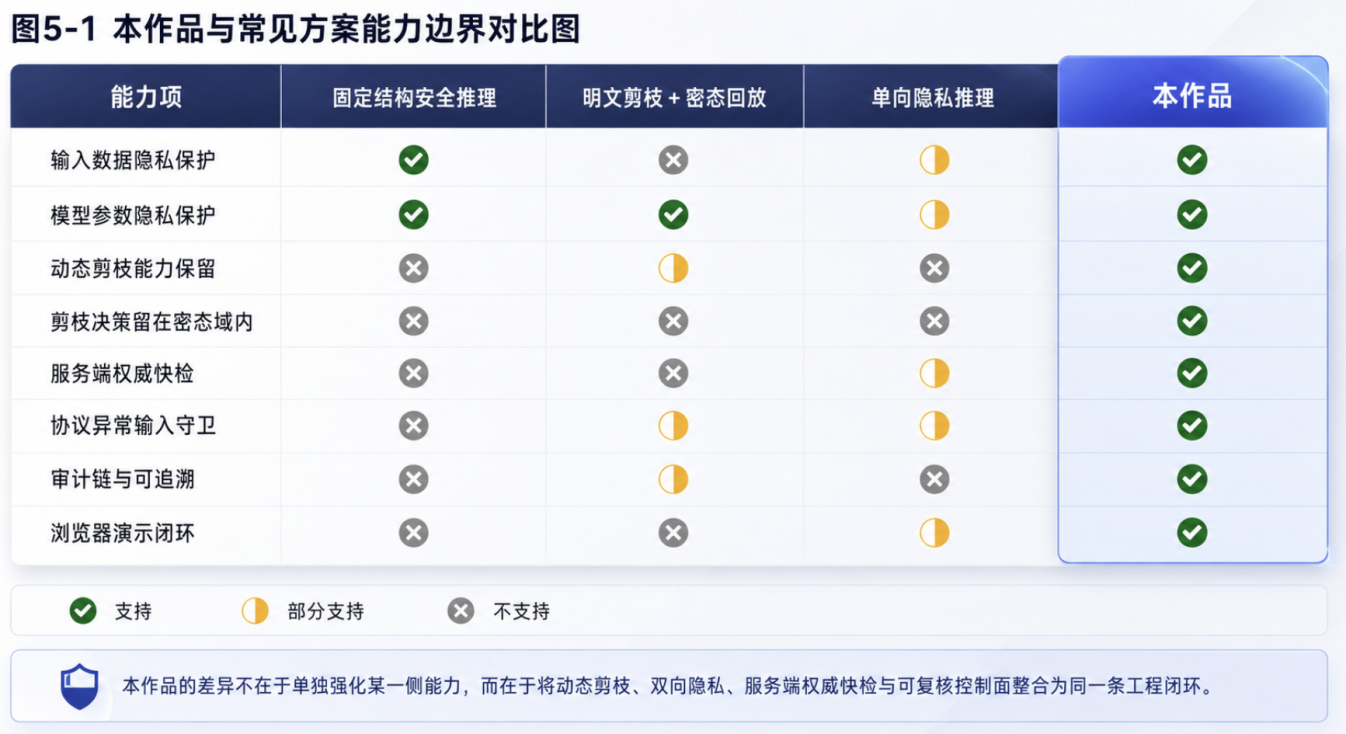
\includegraphics[width=0.92\textwidth]{figures/fig5-1-capability-matrix.jpeg}
\caption{图5-1 本作品与常见方案能力边界对比图：从动态剪枝、双向隐私、服务端快检与可追溯控制面四个维度展示差异。}
\end{figure}

如果把相关方案进一步分类，SecureML[14]、GAZELLE[15]、CrypTen[16] 与 Delphi[17] 更接近通用私有推理系统，它们为线性层、激活函数与模型服务接口提供基础协议与系统支撑；Iron[18]、BOLT[19]、BumbleBee[7] 与 NEXUS[20] 则代表固定结构 Transformer 的协议优化路线，重点降低注意力与非线性算子的执行成本；CipherPrune[21] 进一步把密态词元剪枝与多项式降阶结合起来，试图同时减少后续层 token 规模与近似开销。相比之下，本作品面向的是医疗影像 DynamicViT 场景，强调在两方半诚实模型下保留动态剪枝决策、明确服务端权威快检与审计边界，并为后续医院/模型提供方分离部署保留工程骨架。

从方法边界看，本作品目前选择的是“保留 DynamicViT 语义并进行安全化改写”的路线，而不是重新训练一套专门面向私有推理的 Transformer。其优点是能够直接解释作品与原始动态剪枝模型之间的关系，便于复现和工程交付；限制在于，固定图 keep-mask、排序网络和密态比较会带来额外开销，且尚未利用 CipherPrune[21]、THE-X[22]、MPCFormer[23]、SecFormer[24] 等工作中更激进的多项式化、蒸馏或结构替换策略。因此，当前方案更适合作为可运行的动态安全剪枝基线，而不是效率上限。

\section{当前局限性}

本作品当前仍有六点需要明确说明的边界。第一，当前展示后端采用单进程 Uvicorn/FastAPI 原型承载长耗时 SPU 调用，进入长耗时 SPU 计算后的主动断连感知、任务取消和队列化调度能力仍不完整，因此现有并发守卫不能等价替代生产级拒绝服务防护。第二，当前仓内仅固化了端到端通信量与算子级代理基准证据，未单独落盘医疗动态安全剪枝链路的阶段级时延剖面，因此尚不能给出更细粒度的性能分解。第三，金融任务当前只覆盖 8 条边界压力样本，足以支撑稳定性验证，但不足以单独构成第二应用主线。第四，当前安全模型主要建立在两方半诚实假设上，不覆盖恶意参与方串谋、模型抽取和更强侧信道对抗场景。第五，当前系统尚未系统评估输出结果本身可能带来的反推风险，因此输出侧隐私仍需在后续工作中单独建模与验证。第六，SViT 这类外部对照方案虽然在协议级性能方面表现较优，但仍依赖可信第三方和固定两方执行模型，说明当前隐私保护 ViT 系统在部署角色、信任假设和执行形态上仍存在约束。

此外，当前动态安全剪枝链路虽然已经证明 DynamicViT 安全化重写的可行性，但尚未在统一数据、统一硬件和统一执行边界下系统比较 Iron[18]、BOLT[19]、NEXUS[20]、CipherPrune[21] 等路线的全部收益差异。这意味着本作品当前更适合作为面向医疗影像动态剪枝场景的工程基线，而不是对所有私有 Transformer 方案给出普适最优结论。后续若要充分吸收密态渐进剪枝或非交互协议等新思路，还需要同步调整 keep-mask 生成策略、训练目标、近似算子和部署验证链路。


\chapter{复现与参赛声明}
\section{最低可复现路径}

系统最低可复现验证步骤如表 15 所示。在模型目录与基础 Python 环境已就位的前提下，可在 10–20 分钟内完成最小闭环验证：先启动 Web 演示并在浏览器端加载一张本地医疗样本，确认系统在本地完成预处理与分片后返回分类、质量保障结论、审计摘要与控制面耗时；再运行协议层异常输入脚本与至少一项控制面守卫检查，验证异常输入阻断与并发/重放防护。完整命令与故障排查说明见 \texttt{README\textbackslash\{\}\_REPRODUCE.md}。

\begin{longtable}{>{\raggedright\arraybackslash}p{0.24\textwidth}>{\raggedright\arraybackslash}p{0.24\textwidth}>{\raggedright\arraybackslash}p{0.24\textwidth}>{\raggedright\arraybackslash}p{0.24\textwidth}}
\caption{表 15 系统最低可复现验证步骤}\\
\toprule
\textbf{步骤} & \textbf{预估耗时} & \textbf{入口} & \textbf{预期输出} \\
\midrule
\endfirsthead
\toprule
\textbf{步骤} & \textbf{预估耗时} & \textbf{入口} & \textbf{预期输出} \\
\midrule
\endhead
启动 Web 演示并加载一张本地医疗样本 & 3–8 分钟 & python3 tools/start\_showcase\_spu\_demo.py --host 0.0.0.0 --port 7860 & 浏览器在本地完成预处理与分片后返回分类结果、质量保障结论、审计摘要与控制面耗时 \\
运行协议层异常输入验证 & 2–4 分钟 & python3 tools/showcase\_protocol\_fuzz.py --base-url http://127.0.0.1:7860 & 生成 \texttt{protocol\textbackslash\{\}\_fuzz\textbackslash\{\}\_evidence.json}（或自定义输出文件），验证 multipart/JSON/截断请求体阻断 \\
运行至少一项控制面守卫检查 & 2–6 分钟 & python3 tools/showcase\_guard\_stress.py --base-url http://127.0.0.1:7860 --checks duplicate\_nonce & 验证重复 nonce、重复载荷或并发占满守卫 \\
可选：更换样本重复复核 & 2–5 分钟 & 浏览器重新加载另一张本地样本；或再次运行 python3 tools/showcase\_guard\_stress.py --base-url http://127.0.0.1:7860 --checks duplicate\_nonce & 验证完整计算链路可重复执行，且审计摘要与控制面统计持续生成 \\
\bottomrule
\end{longtable}

从复现层次上看，当前仓库实际上提供了三档入口：第一档是本机展示样例，用于验证浏览器预处理、分片生成与 SPU 分类闭环；第二档是协议层异常输入和控制面守卫验证，用于复核边界阻断与资源状态回落；第三档是真两方部署迁移骨架，用于演练医院侧、模型提供方与协调侧的分角色部署。三档入口共享同一 bundle、阈值口径与证据链文件，目的在于避免“展示链路”“验证链路”“部署链路”彼此割裂。

复现流程强调“结果可验证”而非“环境完全生产化”。本作品保留了本机 SPU 展示样例、服务器复核结果、通信量记录、鲁棒性探针和真实两方部署框架文档，使读者能够分别验证系统是否能运行、关键指标是否有证据、异常输入是否被拦截，以及后续迁移到医院侧与模型提供方分离部署时需要补齐哪些机构配置。该复现边界与第 2.6 节的系统形态划分保持一致。

\section{数据、模型与权重合规声明}

本作品对数据、模型结构与权重文件的分层合规声明与边界说明如表 16所示。作品对数据、模型结构与权重文件分别采用分层合规声明。数据层面，报告与演示不包含真实、未经授权的患者隐私信息；医疗结果仅用于研究验证与竞赛展示，不作为临床诊断依据；金融压力样本仅承担方法边界验证职责。模型层面，公开仓库保留模型结构、运行脚本、图件与报告生成链；权重层面，仓库当前不默认随 Git 分发全部完整权重文件，仅保留必要的 bundle 元数据与加载入口，完整权重需在授权范围内单独提供。

\begin{longtable}{>{\raggedright\arraybackslash}p{0.32\textwidth}>{\raggedright\arraybackslash}p{0.32\textwidth}>{\raggedright\arraybackslash}p{0.32\textwidth}}
\caption{表 16 数据、模型与权重合规边界说明}\\
\toprule
\textbf{对象} & \textbf{当前做法} & \textbf{合规边界} \\
\midrule
\endfirsthead
\toprule
\textbf{对象} & \textbf{当前做法} & \textbf{合规边界} \\
\midrule
\endhead
测试数据 & 仅使用仓内声明范围内的验证数据与压力样本 & 不对外分发未经授权的原始敏感数据 \\
模型结构代码 & 随仓保留并可复现运行链 & 遵循仓内第三方来源与修改映射说明 \\
模型权重 & 默认不随 Git 完整分发，仅保留 bundle 元数据与加载入口 & 需由维护方按授权边界单独提供 \\
第三方预训练/上游组件 & 按原许可证与来源映射保留 & 不对上游本体主张排他性知识产权 \\
\bottomrule
\end{longtable}

\noindent\textit{注：本声明仅适用于本次竞赛提交的原型系统；任何商业使用需单独获得相关数据与模型的授权许可。}

在合规口径上，本作品还区分了“可公开交付物”和“受授权约束资源”两类对象。前者包括代码、报告、图件、验证脚本、公开证据与必要的 bundle 元数据；后者包括完整权重、原始数据集和任何可能恢复真实患者信息或受限模型资产的内容。这样做既是出于竞赛提交的可复核性考虑，也是为了避免将研究验证资产误写为默认可公开再分发资产。

\section{第三方许可、原创边界与技术公开范围}

本作品的知识产权声明按“上游底座、基于 Apache 2.0 的本地适配、团队原创部分”三层边界撰写。报告只描述仓内已实际完成的物理映射，不对未存在的许可证分发项或未落地的文件头声明作超前表述。第三方组件许可与原创边界的物理映射关系如表 17 所示。

\begin{longtable}{>{\raggedright\arraybackslash}p{0.32\textwidth}>{\raggedright\arraybackslash}p{0.32\textwidth}>{\raggedright\arraybackslash}p{0.32\textwidth}}
\caption{表 17 第三方组件许可与原创边界物理映射}\\
\toprule
\textbf{物理映射项} & \textbf{仓内落点} & \textbf{当前事实} \\
\midrule
\endfirsthead
\toprule
\textbf{物理映射项} & \textbf{仓内落点} & \textbf{当前事实} \\
\midrule
\endhead
上游许可证文本 & spu\_vendored/LICENSE & 已保留 Apache License 2.0 文本 \\
vendored 变更总说明 & spu\_vendored/MODIFICATIONS.md & 已列出当前交付版明确引用的本地适配文件 \\
修改文件头声明 1 & spu\_vendored/libspu/spu.proto & 文件头含密捷项目本地修改声明 \\
修改文件头声明 2 & spu\_vendored/libspu/mpc/cheetah/arithmetic.h & 文件头含密捷项目本地供应链适配声明 \\
修改文件头声明 3 & spu\_vendored/libspu/mpc/cheetah/arithmetic.cc & 文件头含密捷项目本地供应链适配声明 \\
修改文件头声明 4 & spu\_vendored/libspu/mpc/cheetah/protocol.cc & 文件头含密捷项目本地供应链适配声明 \\
第三方来源总表 & THIRD\_PARTY.md & 已保留 DynamicViT / OpenBumbleBee 来源与许可证映射 \\
\bottomrule
\end{longtable}

\noindent\textit{注：所有修改文件均已在文件头添加本地修改声明；本作品不对上游开源组件主张任何排他性知识产权。}

本作品的安全计算底座基于 SecretFlow SPU，当前已核对上游分发许可为 Apache License 2.0。当前核对到的上游分发物保留了许可证文件（LICENSE），未发现独立的 NOTICE 分发文件，因此交付物按事实保留许可证文本和本地修改说明，不虚构并不存在的附加分发项。本作品不对上游 SPU、OpenBumbleBee 与相关协议实现本体主张排他性知识产权。

本作品的原创贡献主要集中在动态控制流映射策略、浏览器工作线程控制面、服务端权威快检、前后端审计链闭环、演示程序集成以及报告与图件生成链。当前交付物公开代码、图件、报告与运行脚本；涉及完整模型权重和数据集的部分，按授权边界与来源限制单独管理，不在公开仓库中默认再分发。


\chapter*{参考文献}
\addcontentsline{toc}{chapter}{参考文献}
\begin{thebibliography}{99}
\bibitem{ref1} Dosovitskiy A, Beyer L, Kolesnikov A, et al. An Image is Worth 16x16 Words: Transformers for Image Recognition at Scale[C]//International Conference on Learning Representations (ICLR). 2021.
\bibitem{ref2} Rao Y, et al. DynamicViT: Efficient Vision Transformers with Dynamic Token Sparsification[C]//Advances in Neural Information Processing Systems (NeurIPS). 2021.
\bibitem{ref3} Zeng W, et al. MPCViT: Searching for Accurate and Efficient MPC-Friendly Vision Transformer with Heterogeneous Attention[C]//Proceedings of the IEEE/CVF International Conference on Computer Vision (ICCV). 2023.
\bibitem{ref4} Touvron H, Cord M, Douze M, Massa F, Sablayrolles A, Jégou H. Training data-efficient image transformers \& distillation through attention[C]//Proceedings of the 38th International Conference on Machine Learning (ICML). 2021.
\bibitem{ref5} Huang G, Liu Z, van der Maaten L, Weinberger K Q. Densely Connected Convolutional Networks[C]//Proceedings of the IEEE Conference on Computer Vision and Pattern Recognition (CVPR). 2017.
\bibitem{ref6} Ma J, et al. SecretFlow-SPU: A Performant and User-Friendly Framework for Privacy-Preserving Machine Learning[C]//USENIX Annual Technical Conference (USENIX ATC). 2023.
\bibitem{ref7} Lu W, et al. BumbleBee: Secure Two-party Inference Framework for Large Transformers[C]//Network and Distributed System Security Symposium (NDSS). 2025.
\bibitem{ref8} Batcher K E. Sorting Networks and Their Applications[C]//Proceedings of the AFIPS Spring Joint Computer Conference. 1968: 307-314.
\bibitem{ref9} Yao A C. Protocols for Secure Computations[C]//23rd Annual Symposium on Foundations of Computer Science (FOCS). 1982: 160-164.
\bibitem{ref10} Masinter L. Returning Values from Forms: multipart/form-data[S]. RFC 7578. IETF, 2015.
\bibitem{ref11} National Institute of Standards and Technology. Secure Hash Standard (SHS)[S]. FIPS PUB 180-4. Gaithersburg, MD: NIST, 2015.
\bibitem{ref12} WHATWG. HTML Living Standard: Web Workers[EB/OL]. https://html.spec.whatwg.org/dev/workers.html, 2026-05-20.
\bibitem{ref13} 马敏, 付钰, 黄凯, 贾潇风. 基于秘密共享的轻量级隐私保护ViT推理框架[J]. 通信学报, 2024, 45(4): 27-38. DOI:10.11959/j.issn.1000-436x.2024025.
\bibitem{ref14} Mohassel P, Zhang Y. SecureML: A System for Scalable Privacy-Preserving Machine Learning[C]//2017 IEEE Symposium on Security and Privacy (SP). 2017: 19-38.
\bibitem{ref15} Juvekar C, Vaikuntanathan V, Chandrakasan A. GAZELLE: A Low Latency Framework for Secure Neural Network Inference[C]//27th USENIX Security Symposium (USENIX Security). 2018: 1651-1669.
\bibitem{ref16} Knott B, Venkataraman S, Hannun A, et al. CrypTen: Secure Multi-Party Computation Meets Machine Learning[C]//Advances in Neural Information Processing Systems (NeurIPS). 2021.
\bibitem{ref17} Mishra P, Lehmkuhl R, Srinivasan A, Zheng W, Popa R A. Delphi: A Cryptographic Inference Service for Neural Networks[C]//29th USENIX Security Symposium (USENIX Security). 2020: 2505-2522.
\bibitem{ref18} Hao M, Li H, Chen H, et al. Iron: Private Inference on Transformers[C]//Advances in Neural Information Processing Systems (NeurIPS). 2022.
\bibitem{ref19} Pang Q, Zhu J, Möllering H, Zheng W, Schneider T. BOLT: Privacy-Preserving, Accurate and Efficient Inference for Transformers[C]//2024 IEEE Symposium on Security and Privacy (SP). 2024.
\bibitem{ref20} Zhang J, Yang X, He L, et al. Secure Transformer Inference Made Non-interactive[C]//Network and Distributed System Security Symposium (NDSS). 2025.
\bibitem{ref21} Zhang Y, Xue J, Zheng M, et al. CipherPrune: Efficient and Scalable Private Transformer Inference[C]//International Conference on Learning Representations (ICLR). 2025.
\bibitem{ref22} Chen T, Bao H, Huang S, et al. THE-X: Privacy-Preserving Transformer Inference with Homomorphic Encryption[C]//Findings of the Association for Computational Linguistics: ACL 2022. 2022: 3510-3520. DOI:10.18653/v1/2022.findings-acl.277.
\bibitem{ref23} Li D, Shao R, Wang H, et al. MPCFormer: Fast, Performant and Private Transformer Inference with MPC[C]//International Conference on Learning Representations (ICLR). 2023.
\bibitem{ref24} Luo J, Zhang Y, Zhang Z, et al. SecFormer: Fast and Accurate Privacy-Preserving Inference for Transformer Models via SMPC[C]//Findings of the Association for Computational Linguistics: ACL 2024. 2024: 13333-13348. DOI:10.18653/v1/2024.findings-acl.790.
\bibitem{ref25} Liu J, Juuti M, Lu Y, Asokan N. Oblivious Neural Network Predictions via MiniONN Transformations[C]//Proceedings of the 2017 ACM SIGSAC Conference on Computer and Communications Security (CCS). 2017: 619-631.
\bibitem{ref26} Riazi M S, Samragh M, Chen H, Laine K, Lauter K, Koushanfar F. XONN: XNOR-based Oblivious Deep Neural Network Inference[C]//28th USENIX Security Symposium (USENIX Security). 2019: 1501-1518.
\bibitem{ref27} Liang Y, Ge C, Tong Z, Song Y, Wang J, Xie P. EViT: Expediting Vision Transformers via Token Reorganizations[C]//International Conference on Learning Representations (ICLR). 2022.
\bibitem{ref28} Yin H, Vahdat A, Alvarez J M, Mallya A, Kautz J, Molchanov P. A-ViT: Adaptive Tokens for Efficient Vision Transformer[C]//Proceedings of the IEEE/CVF Conference on Computer Vision and Pattern Recognition (CVPR). 2022: 10809-10818. DOI:10.1109/CVPR52688.2022.01054.
\bibitem{ref29} Bolya D, Fu C-Y, Dai X, Zhang P, Feichtenhofer C, Hoffman J. Token Merging: Your ViT But Faster[C]//International Conference on Learning Representations (ICLR). 2023.
\end{thebibliography}


\ifincludeappendix
  \appendix
  \renewcommand{\thesection}{\Alph{chapter}.\arabic{section}}
  \chapter{关键代码实现}
  本附录不再罗列完整源文件，而是按“公式—机制—证据”对应关系摘录最能代表系统实现要点的局部代码，用于说明浏览器端 little-endian share 序列化、SPU 内部安全排序与 keep-mask 构造、结构化元数据长度门以及黑盒 fuzz 用例构造等核心实现。

\section{浏览器 Worker 中的 little-endian share 序列化}

代码位置：showcase/src/workers/medicalControlPlaneWorker.ts:148

该段代码展示了浏览器 Worker 如何显式使用 little-endian 方式写入 Float32 share，避免异构环境的字节序歧义。

以下仅保留与正文论证直接相关的关键代码节选，已省略无关分支、重复检查与通用异常处理。

\begin{lstlisting}
function packFloat32LE(values) {
  const bytes = new Uint8Array(values.length * 4);
  const view = new DataView(bytes.buffer);
  for (let index = 0; index < values.length; index += 1) {
    const value = values[index];
    if (!Number.isFinite(value)) throw new Error(`Non-finite float at ${index}`);
    view.setFloat32(index * 4, Math.fround(value), true);
  }
  return bytes;
}
\end{lstlisting}

\section{安全选择与双调排序的核心 SPU 实现}

代码位置：integrations/transshield\_runtime/e2e\_secure\_vit/spu\_static\_vit.py:639

该段代码展示了 JAX/SPU 路径如何通过编码键、按索引跟踪的双调排序和向量化 keep-mask 构造，稳定处理安全 Top-与并列分数决断问题。

以下仅保留与正文论证直接相关的关键代码节选，已省略无关分支、重复检查与通用异常处理。

\begin{lstlisting}
def _bitonic_sort_desc_with_indices(values):
    indices = jnp.broadcast_to(jnp.arange(N, dtype=jnp.int32), values.shape)
    ...
    left_index = jnp.where(is_left, p_arr, p_partner)
    is_desc = (left_index & k) == 0
    ...
    indices = jnp.where(has_partner, new_idx, indices)
    return x, indices

def _secure_build_keep_decision(score, prev_decision_2d, keep_count):
    active_before = prev_decision_2d.squeeze(-1) > 0
    encoded_key = score - jnp.arange(N, dtype=score.dtype) * 1e-6
    encoded_masked = jnp.where(active_before, encoded_key, float('-inf'))
    ...
    sorted_keys, sorted_indices = _bitonic_sort_desc_with_indices(sortable)
    top_k_indices = sorted_indices[:, :keep_count]
    keep_mask = jnp.any(top_k_indices[:, :, None] == pos[None, None, :], axis=1)
    return (keep_mask[:, :N] & active_before)[:, :, None]
\end{lstlisting}

\section{JSON 字节长度门与 strict json.loads 钩子}

代码位置：showcase\_api/control\_plane.py:309

该段代码展示了在 \texttt{json.loads} 前先执行字节长度门，并为整数、浮点和常量解析分别挂接严格钩子。

以下仅保留与正文论证直接相关的关键代码节选，已省略无关分支、重复检查与通用异常处理。

\begin{lstlisting}
def _load_json_part(self, raw_body: bytes, part: RawPart):
    part_view = memoryview(raw_body)[part.body_start:part.body_end]
    body_len = len(part_view)
    if body_len > JSON_PART_MAX_BYTES:
        raise ValueError('json part exceeds global size limit')
    field_limit = {...}.get(part.name, JSON_PART_MAX_BYTES)
    if body_len > field_limit:
        raise ValueError(f'{part.name} exceeds field size limit')
    decoded = bytes(part_view).decode('utf-8', 'strict')
    return json.loads(decoded, parse_int=strict_json_int,
                      parse_float=strict_json_float,
                      parse_constant=strict_json_constant)
\end{lstlisting}

\section{协议层异常输入黑盒验证样例}

代码位置：tools/showcase\_protocol\_fuzz.py:158

该段代码展示了针对 畸形 multipart header的黑盒测试用例，以及脚本对拦截层级和资源状态的记录方式。

以下仅保留与正文论证直接相关的关键代码节选，已省略无关分支、重复检查与通用异常处理。

\begin{lstlisting}
def case_header_null_byte(base_url: str, timeout: float, server_pid: int | None):
    boundary = f'nullbyte-{uuid.uuid4().hex}'
    header = (
        b'Content-Disposition: form-data; '
        b'name="domai\x00n"'
    )
    body = build_custom_body(boundary, header, b'medical')
    raw = build_raw_multipart_request(
        base_url, boundary_param=f'boundary={boundary}', body=body
    )
    return capture_case(
        name='multipart_header_null_byte_blocked',
        action=lambda: send_raw_http(base_url, raw, timeout),
        interception_layer='multipart_header_parser',
        fallback_layer='mime_tree_validation',
    )
\end{lstlisting}

\fi

\end{document}
